%% ---------------------------------------------------------------
%%              Trabalho de conclusão de curso - Latex
%%
%%      UNICAMP - Faculdade de Engenharia Mecânica
%%       
%%      2019
%%		
%% ---------------------------------------------------------------

%Quando for imprimir, mude os comandos de \clearpage para \cleardoublepage, pois assim quando mandar pra impressora não terá problemas ao imprimir frente e verso (basta apagar \clearpage e habilitar o \cleardoublepage que está como comentário). 

% Especificação da classe do documento
\documentclass[12pt,twoside]{report}
%A classe "report" é utilizada para documentos que possuem capitulos, pequenos livros, tese... 
%"twoside" indica que o documento sera impresso frente e verso. Note que isso não ira comunicar a impressora para imprimir desse modo. 

% Inserção dos pacotes e possíveis comandos a serem utilizados durante a escrita
% -----------------------------------------------------------------------------
%                                      PACOTES PRINCIPAIS
% -----------------------------------------------------------------------------

%% Codificação e formatação básica do LaTeX
% Dimensoes da pagina
\usepackage[paperheight=297mm,paperwidth=210mm,top=3cm,left=3cm,right=2cm,bottom=2cm]{geometry}    % Dimensões da página (A4)
\usepackage[portuges, brazilian]{babel} % Hiphenação em portugues
\usepackage[utf8]{inputenc}             % Codificação do arquivo
\usepackage[T1]{fontenc}
\usepackage{uarial}                      % Pacote de fonte Times
\usepackage{lhelp}                      % Denine macros úteis
\usepackage{ccaption}                   % Opções para capítulos
\usepackage{indentfirst}                % Identação do primeiro parágrafo
\usepackage{fancyhdr}                   % Controlar os cabeçalhos e rodapés
\usepackage{enumerate}                  % Para usar enumerações
\usepackage{cmap}                       % Mapear caracteres especiais no PDF

\usepackage{floatflt}                   % Quebra de texto em figuras e tabelas
\usepackage{colortbl}                   % Adicionar cor às tabelas
\usepackage{fancyvrb}                   % Texto verbatim sofisticado
\usepackage{wrapfig}                    % Produz figuras que o texto pode ficar ao redor
\usepackage{url}                        % Adiciona URLs
\usepackage{multirow}                   % Permite construir células multi-linhas

% Essencial para colocar funções e outros símbolos matemáticos
\usepackage{amsmath, amssymb, amsthm}
\usepackage{amscd, amsfonts, textcomp}
\usepackage{psfrag,layout}

% Links dinâmicos
% Suporte para hipertexto, links para referências e figuras

% To Dvi.
%\usepackage[dvipdfmx,plainpages=false,pdfpagelabels,colorlinks=true,
%citecolor=black,linkcolor=black,urlcolor=black,filecolor=black,
%bookmarksopen=true]{hyperref}

% To pdflatex
\usepackage[pdftex, plainpages=false, pdfpagelabels, colorlinks=true,
citecolor=black,linkcolor=black, urlcolor=black, filecolor=black,
bookmarksopen=true]{hyperref}

\usepackage[dvipsnames,svgnames,table]{xcolor}
\usepackage{pdfpages}			% Inclui paginas em pdf no arquivo
\usepackage{epstopdf}			% Converte figuras em formato eps para pdf
\usepackage{color}				% Suporte para cores
\usepackage{transparent}		% Suporte para vários conjuntos de cores
\usepackage{siunitx}			% Sistema internacional de unidades
\usepackage{lipsum}

\usepackage[all]{hypcap}                % Soluciona o problema com o hyperref e capítulos
\usepackage{wasysym}                    % Símbolos especiais com \female e \male etc.
\usepackage{bigstrut}                   % Espaçamento na tabela
\usepackage{comment}                    % Comentar várias linhas simultâneas
\usepackage{epigraph}                   % Epígrafe
\usepackage[titles,subfigure]{tocloft}  % Permite formatar o sumário
\usepackage{makeidx}
\usepackage{emptypage}					 % Retira o número de páginas em branco
\usepackage{afterpage}
\usepackage{kantlipsum}					 % mock text
\usepackage{setspace}                   % Para definir espaçamento entre as linhas
\usepackage{listings}                   % Para Inserir código fonte
\usepackage{mathtools, nccmath}         % Para alinhamento e redução na fonte de equações

% -----------------------------------------------------------------------------
%                                       ELEMENTOS GRÁFICOS
% -----------------------------------------------------------------------------
\usepackage{graphics}                   % Suporte padrão para gráficos
\usepackage{graphicx}                   % Suporte avançado para gráficos
\usepackage[]{graphicx}                 % Para incluir figuras (pacote extendido)
\usepackage[normalsize]{subfigure}      % Possibilita a utilização de subfiguras
% \usepackage{subfig}                     % Criar figura dividida em subfiguras
\usepackage{epsfig}                     % Uso de figuras eps.
\usepackage{epsf}

\usepackage{caption}                    % Customizar as legendas de figuras e tabelas
\usepackage{multicol}                   % Criar ambientes com 2 ou mais colunas
% -----------------------------------------------------------------------------
% Pacotes para Tabelas
\usepackage{array}                      % Elementos extras para formatação de tabelas
\usepackage{booktabs}                   % Tabelas com qualidade de publicação
\usepackage{longtable}                  % Para criar tabelas maiores que uma página
\usepackage{lscape}                     % adicionar tabelas e figuras como landscape

%% Lista de Abreviações
% \usepackage[notintoc,portuguese]{nomencl}   % Cria lista de abreviações
\usepackage{nomencl}
\makenomenclature

% %  Lista de Tabela de siglas e simbolos.
%\usepackage{tabela-simbolos} 
% %  Letras maiúsculas são colocados antes dos símbolos de minúsculas.
%\usepackage[caixa=Mm]{tabela-simbolos}
% %  Define a ordem em que vai aparecer os simbolos, as letras gregas e romanas.
%\usepackage[romanos=2,gregos=3,simbolos=1]{tabela-simbolos}

%% Notas de rodapé
\usepackage{footnote}                   % Lidar com notas de rodapé em diversas situações
\makesavenoteenv{tabular}               % Notas criadas nas tabelas ficam no fim das tabelas
\usepackage{pifont}                     % Acesso a PostScript Symbol padrão e fontes Dingbats
\usepackage{lastpage}                   % Conta o número de páginas
\usepackage{ifoddpage}				 % Inclui n de páginas impares.
\newcommand\alwaysodd[1]{%
  \checkoddpage
  \ifoddpage
    #1%
  \else
    \mbox{}\clearpage#1%
  \fi
}

%% Referências bibliográficas e afins
%\usepackage[round]{natbib}              % Citações tipo (nome-ano)
%\usepackage{natbib}                    % Citações tipo [nome-ano]

% Adicionar bibliografia, índice e conteúdo na Tabela de conteúdo
% Não inclui lista de tabelas e figuras no índice
\usepackage[nottoc,notlof,notlot]{tocbibind}

%% Pontuação e unidades
\usepackage{icomma}		% Posicionar inteligentemente a vírgula como separador decimal
\usepackage[tight]{units}	% Formatar as unidades com as distâncias corretas
% -----------------------------------------------------------------------------
%                                   FORMATAÇÕES DE TEXTO
% -----------------------------------------------------------------------------
\usepackage{parskip}					% Espaçamento entre paragrafos
%\special{papersize=210mm,297mm}    		% Tamanho do papel (neste caso papel A4)
\pagenumbering{roman}                   % Numeração das paginas iniciais em romano
\setlength{\parindent}{1cm}             % Parágrafo de 1cm
% \setlength{\mathindent}{1cm}          % Indentação das fórmulas matemáticas
\setlength{\fboxsep}{1mm}               %   Espaçamento do texto para o frame, também define
                                        % espaçamento entre colunas da tabela
                                        
\frenchspacing                          % Não põe um espaço adicional após ponto final
\sloppy                                 % Força que todas as linhas fiquem dentro das margens
\raggedbottom                           % Para não permitir espaços extra no texto
\def\figurename{Figura.}                % Define como a palavra figura será escrito
\def\tablename{Tabela.}                 % Define como a palavra tabela será escrito

\newcommand{\eq}[1]{Equação~(\ref{#1})}	% Facilita a citação de Equações
\newcommand{\figu}[1]{Figura~\ref{#1}}		% Facilita a citação de Figuras
\newcommand{\tab}[1]{Tabela~\ref{#1}}		% Facilita a citação de Tabelas

% Citação tipo (AUTOR, ano), conforme ABNT
%\renewcommand{\cite}[1]{{\citeauthor{#1},~\citeyear{#1}}}
%\renewcommand{\citep}[1]{(\citeauthor{#1},~\citeyear{#1})}
%\renewcommand{\citet}[1]{\citeauthor{#1}}

%
\theoremstyle{definition}
\newtheorem{defi}{Definição}[chapter]		% Para introduzir uma definição
\newtheorem{teo}{Teorema}[chapter]		% Para introduzir um teorema
\newcommand{\nomunit}[1]{%
\renewcommand{\nomentryend}{\dotfill[#1]}}	% Colocar unidades na lista de Abreviaturas e siglas

%% Estes comandos criam os subgrupos na Lista de Abreviaturas e Siglas
\renewcommand{\nomgroup}[1]{%
  \ifthenelse{\equal{#1}{A}}{\item[\textbf{Letras Latinas}]}{\hrulefill%			a
    \ifthenelse{\equal{#1}{C}}{\item[\textbf{Letras Gregas}]}}}}				c
        \ifthenelse{\equal{#1}{G}}{\item[\textbf{Subscritos}]}}}}}}			e
           \ifthenelse{\equal{#1}{K}}{\item[\textbf{Siglas}]}{}}{}}{}}{}}{}}{}}%		f
%
\setcounter{secnumdepth}{5}	% Serve pra introduzir um quinto nível de seções (subsubsubsection)
\setcounter{tocdepth}{5}	% Serve pra introduzir um quinto nível de seções (subsubsubsection)
%
\makeatletter			% Changes the category code of '@' character to 11
% -----------------------------------------------------------------------------
%                                          OPERADORES
% -----------------------------------------------------------------------------
% Conforme a necessidade de cada trabalho
\newcommand{\vectornorm}[1]{\left|\left|#1\right|\right|}   % Facilita a introdução da norma ||w||
\newcommand{\argmax}{\operatornamewithlimits{argmax}}       % Facilita a escrita de argmax
\newcommand{\latex}{\LaTeX~}                                % Facilita a escrita de LaTeX
\newlength\figureheight
\newlength\figurewidth
% -----------------------------------------------------------------------------
%                             FORMATANDO SEÇÕES, TABELAS E EQUAÇÕES
% -----------------------------------------------------------------------------
\@addtoreset{figure}{chapter}
\renewcommand{\thefigure}{\thechapter.\@arabic\c@figure}

\@addtoreset{equation}{chapter}
\renewcommand{\theequation}{\thechapter.\@arabic\c@equation}

\@addtoreset{table}{chapter}
\renewcommand{\thetable}{\thechapter.\@arabic\c@table}

\def\chapter{\@startsection{chapter}{1}
          {\z@}{26pt minus 0pt}{12pt minus 0pt}{\renewcommand{\rmdefault}{phv}\large\bf}}
\def\appendix{\@startsection{chapter}{1}
          {\z@}{26pt minus 0pt}{12pt minus 0pt}
          {\large{\textsf{\textbf{APÊNDICE}}}~~\renewcommand{\rmdefault}{phv}\large\bf}}
\def\section{\@startsection{section}{2}
          {\z@}{26pt minus 0pt}{12pt minus 0pt}{\renewcommand{\rmdefault}{phv}\bf}}
\def\subsection{\@startsection{subsection}{3}
          {\z@}{26pt minus 0pt}{12pt minus 0pt}{\renewcommand{\rmdefault}{phv}\bf}}
\def\subsubsection{\@startsection{subsubsection}{4}
          {\z@}{26pt minus 0pt}{12pt minus 0pt}{\renewcommand{\rmdefault}{phv}\bf}}
\def\subsubsubsection{\@startsection{subsubsubsection}{5}
          {\z@}{26pt minus 0pt}{12pt minus 0pt}{\renewcommand{\rmdefault}{phv}\bf}}
         
\newcounter {anexo}[chapter]
\def\anexo{\@startsection{chapter}{1}
          {\z@}{26pt minus 0pt}{12pt minus 0pt}
	  {\large{\textsf{\textbf{ANEXO}}}~~\renewcommand{\rmdefault}{phv}\large\bf}}

% -----------------------------------------------------------------------------
%                                         SUB-SUB-SUB-SECTION
% -----------------------------------------------------------------------------
\newcounter {subsubsubsection}[subsubsection]
\renewcommand\thesubsubsubsection{}
% \newcommand\subsubsubsection{\@startsection{subsubsubsection}{4}{\z@}%
%                             {12pt minus 0pt}{12pt minus 0pt}{\normalfont\normalsize\it}}
% Espaçamento do numero da subsubsubseção em relação à marge no sumário.
\newcommand*\l@subsubsubsection{\@dottedtocline{3}{8em}{2.2em}}
\newcommand*{\subsubsubsectionmark}[1]{}

% -----------------------------------------------------------------------------

\def\thechapter{\arabic{chapter}}
\def\thesection{\thechapter.\arabic{section}}	
\def\thesubsection{\thesection.\arabic{subsection}}
% \def\thesubsubsection{\Alph{subsubsection}}
\def\thesubsubsection{}
\makeatother				% Reverts (\makealetter) this to its original catcode of 12.

%\renewcommand\cftsecfont{\bf}                % Títulos das seções em negrito no sumário
%\renewcommand{\cftsecleader}{\cftdotfill{\cftnodots}}  % Elimina os pontos na frente das seções no sumário
%\setlength\cftbeforesecskip{12pt}            % Espaçamento antes da seção no sumário
%\renewcommand{\cftsecindent}{0 em}           % Espaçamento do numero da seção em relação à marge no sumário
%\renewcommand{\cftsecnumwidth}{1.9 em}       % Espaçamento do título da seção em relação ao número no sumário
%\renewcommand{\cftsubsecindent}{1.9 em}      % Espaçamento do numero da subseção em relação à marge no sumário
%\renewcommand{\cftsubsecnumwidth}{2.8 em}    % Espaçamento do título da subseção em relação ao número no sumário
%\renewcommand{\cftsubsubsecindent}{4.7 em}   % Espaçamento do numero da subsubseção em relação à marge no sumário
\renewcommand{\cftsubsubsecnumwidth}{1.9 em}  %     Espaçamento do título da subsubseção em relação
                                              % ao número no sumário



% -----------------------------------------------------------------------------
%                                     ESTILOS DO PACOTE FANCYHDR
% -----------------------------------------------------------------------------
% Usar os estilos do pacote fancyhdr
\pagestyle{fancy}
\fancypagestyle{plain}{\fancyhf{}}
\fancyhead{}                                % Limpar os campos do cabeçalho atual
% Número da página do lado esquerdo [L] nas páginas ímpares [O] e do lado direito [R] nas páginas pares [E]
%\fancyhead[LO,RE]{\thepage}
%\fancyhead[RO]{\nouppercase{\rightmark}}   % Nome da seção do lado direito em páginas ímpares
%\fancyhead[LE]{\nouppercase{\leftmark}}    % Nome do capítulo do lado esquerdo em páginas pares
\fancyfoot{}                                % Limpar os campos do rodapé
\fancyfoot[CO, CE]{\thepage}
\renewcommand{\headrulewidth}{0pt}          % Omitir linha de separação entre cabeçalho e conteúdo
\renewcommand{\footrulewidth}{0pt}          % Omitir linha de separação entre rodapé e conteúdo
\headheight 14.5pt                          % Altura do cabeçalho



% -----------------------------------------------------------------------------
%                                        COMANDOS CUSTOMIZADOS
% -----------------------------------------------------------------------------
%  Ambiente para criar exemplos dentro de um capítulo.
\usepackage{verbatim}
\usepackage{float}
\usepackage{graphicx,subfigure}
\floatstyle{boxed}
\newfloat{program}{!th}{lop}
\floatname{program}{Exemplo}

\newbox\examplebox
\newenvironment{example}[2]{%
    \program
    \vskip-.7\baselineskip
    \caption{#2}%
    \label{#1}%
    \verbatim
}{%
    \endverbatim
    \vskip-.7\baselineskip
    \endprogram
}
\numberwithin{program}{chapter}

%% Redefinição de marcadores.
% Types of itemize
% \circ — An open circle
% \cdot — A centered dot
% \star — A five-pointed star
% \ast — A centered asterisk
% \rightarrow — A short right-pointing arrow
% \diamondsuit — An open diamond
\renewcommand{\labelitemi}{$\circ$}
\renewcommand{\labelitemii}{$\cdot$}
\renewcommand{\labelitemiii}{$\diamond$}
\renewcommand{\labelitemiv}{$\ast$}




\begin{document}
% -----------------------------------------------------------------------------
%                                   ARQUIVOS DA DISSERTAÇÃO
% -----------------------------------------------------------------------------
% Capa, prefácio, abstract e afins

% -----------------------------------------------------------------------------
%                                CAPA DO TRABALHO
% -----------------------------------------------------------------------------

%Quando for imprimir, mude os comandos de \clearpage para \cleardoublepage, pois assim quando mandar pra impressora não terá problemas ao imprimir frente e verso (basta apagar \clearpage e habilitar o \cleardoublepage). 

\thispagestyle{fancy}
\fancyhf{}
\lhead{
  \begin{picture}(225,150)%(horizontal,vertical)
    \put(0,0){
\includegraphics[scale=0.13]{pre/logo-unicamp.jpg}}
  \end{picture}
}
\cfoot{} 

\begin{center}
\vspace*{5cm}
{\fontsize{14}{14} \textbf{UNIVERSIDADE ESTADUAL DE CAMPINAS}}	\\ 
\vspace{0.6ex}
{\fontsize{14}{14} \textbf{Faculdade de Engenharia Mecânica}}	\\ 
\vspace{3cm}
%{\fontsize{12}{12} \textbf{Relatório Parcial}}	\\ 
{\fontsize{12}{12} \textbf{Trabalho de Conclusão de Curso}}	\\
\vspace{3cm}
{\fontsize{23}{23} \textbf{Simulação da Mão Humana Utilizando o Modelo de Hill Simplificado}}\\
\vspace{1.6ex}
{\fontsize{23}{23} \textbf{}}\\ 
\end{center}
\vspace{3cm}
\begin{flushright}
{\fontsize{12}{12} \textbf{Autor: Giovani Valencise}}\\ 
{\fontsize{12}{12} \textbf{Orientador: Prof. Dr. Eric Fujiwara}}\\
\end{flushright}
\vspace{2cm}
\begin{center}
CAMPINAS\\ 
2019
\end{center}


% -----------------------------------------------------------------------------
%                              ASSINATURA DO ORIENTADOR
% -----------------------------------------------------------------------------
%\cleardoublepage - habilite para imprimir
\clearpage
\thispagestyle{plain}



\begin{center}
\vspace*{0.8cm}

{\fontsize{14}{14} \textbf{UNIVERSIDADE ESTADUAL DE CAMPINAS}}	\\
{\fontsize{14}{14} \textbf{FACULDADE DE ENGENHARIA MECÂNICA}}	\\

\vspace{3cm}
%{\fontsize{12}{12} \textbf{Relatório Parcial}}	\\ 
{\fontsize{12}{12} \textbf{Trabalho de Conclusão de Curso}}	\\
\vspace{3cm}
{\fontsize{23}{23} \textbf{Simulação da Mão Humana Utilizando o Modelo de Hill Simplificado}}\\
\end{center}

\vspace*{2cm}
\begin{flushleft}
Trabalho de Conclusão de Graduação apresentada à Faculdade de Engenharia Mecânica da Universidade Estadual de Campinas como parte dos requisitos exigidos para obtenção do título de Engenheiro no curso de Engenharia de Controle e Automação.
\end{flushleft}

\vspace*{0.5cm}



\vspace{0.5cm}
\noindent
Autor: Giovani Valencise\\
Orientador: Prof. Dr. Eric Fujiwara	\\


\vspace{0.6cm}

\vspace{4.0cm}
\begin{center}
\textbf{CAMPINAS}\\ 
\textbf{2019}
\end{center}


% % -----------------------------------------------------------------------------
% %                                     FICHA CATALOGRÁFICA
% % -----------------------------------------------------------------------------
% \newpage %essa parte deve estar atrás da contra capa, logo não precisa colocar o comando \cleardoublepage

% \begin{center}
% \begin{tabular}{c}
%   FICHA CATALOGRÁFICA ELABORADA PELA \\
%   BIBLIOTECA DA ÁREA DE ENGENHARIA E ARQUITETURA - BAE - UNICAMP \\
% \end{tabular}
% \end{center}

% \vspace{0.8cm}
% \begin{tabular}{|cl|} 
% 	\hline
% 	&Agência(s):\\
% 	&Nº do Proc.:\\
% 	\hline	
% \end{tabular}
%-----------------------------------------------------------------------------
% Essa parte é feita pela BAE, você terá que incluir a página feita por eles com o comando "input" pdf. A tabela seguinte é um exemplo. Veja a observação 2 antes de retirar o comentario. Note que não foi centralizada, para fazer isso e so deslocar o comando \end{center} acima. 

%\begin{tabular}{|cl|} \hline
%  \hspace{2cm} & \\
%  & Penteado, Marcos Roberto Mendes, 1985-				\\  
%  P387t & \hspace{0.15in} Transporte de grãos por leito móvel em um escoamento turbulento :\\
%  & deslocamento de grãos individuais / Marcos Roberto Mendes Penteado. –\\
%  & Campinas, SP : [s.n.], 2015.\\
%  &  \\  
%  & \hspace{0.15in} Orientador: Erick de Moraes Franklin.\\
%  & \hspace{0.15in} Dissertação (mestrado) – Universidade Estadual de Campinas, Faculdade de\\
%  & Engenharia Mecânica. \\
%  & \\
%  & \hspace{0.15in} 1. Transporte de sedimentos. 2. Escoamento turbulento. 3. Tratamento de\\
%  & imagens. I. Franklin, Erick de Moraes,1974-. II. Universidade Estadual de\\
%  & Campinas. Faculdade de Engenharia Mecânica. III. Título.\\
%  & \\ \hline
%\end{tabular}
%-----------------------------------------------------------------------------

% \vspace{1.8cm}
% \textcolor{Blue}{Obs. 1. Quando se tratar de Teses e Dissertações financiadas por agências de fomento, os beneficiados deverão fazer referência ao apoio recebido e inserir esta informação na Ficha Catalográfica, além do nome da agência, o número do processo pelo qual recebeu o Auxílio.}\\

% \vspace{0.8cm}
% \textcolor{Blue}{Obs 2. Alunos bolsistas favor solicitarem esse número na CPG/FEM.}\\

% \vspace{0.8cm}
% \textcolor{Blue}{Obs. 3. Caso a tese de doutorado seja feita em Cotutela, será necessário informar na ficha catalográfica o fato, a Universidade convenente, o País e o nome do Orientador/Coorientador.}\\

\fancyhead{}	% Limpa os campos do cabeçalho atual

% % -----------------------------------------------------------------------------
% %                                     FOLHA DE APROVAÇÃO
% % -----------------------------------------------------------------------------
% %\cleardoublepage
% \clearpage
% \begin{center}


% {\large\textbf{UNIVERSIDADE ESTADUAL DE CAMPINAS\\\vspace{1.2ex}
% FACULDADE DE ENGENHARIA MECÂNICA\\\vspace{1.2ex}
% COMISSÃO DE GRADUAÇÃO EM ENGENHARIA DE CONTROLE E AUTOMAÇÃO\\\vspace{1.2ex}
% }}

% \vspace{0.7cm}
% \textbf{TESE DE CONCLUSÃO DE GRADUAÇÃO}

% \vspace{1.2cm}
% {\fontsize{23}{23} \textbf{Aplicação de redes neurais e aprendizado de máquina para agrupamento de bases de dados de forma inteligente}}\\
% \vspace{1.6ex}
% {\fontsize{23}{23} \textbf{}}\\ 

% \begin{flushleft}
% \vspace{0.4cm}
% Autor: Bruno de Souza Ferreira\\
% \vspace{0.2cm}
% Orientador: Prof. Dr. Eric Fujiwara\\


% \vspace{0.3cm}
% A Banca Examinadora composta pelos membros abaixo aprovou esta Tese:  \\

% \vspace{0.5cm}
% \noindent\rule{10cm}{0.4pt}\\
% \textbf{Prof. Dr.\\
% Instituição \\}

% \vspace{0.4cm}
% \noindent\rule{10cm}{0.4pt}\\
% \textbf{Prof. Dr.\\
% Instituição \\}

% \vspace{0.4cm}
% \noindent\rule{10cm}{0.4pt}\\
% \textbf{Prof. Dr.\\
% Instituição \\}

% \vspace{0.4cm}
% \noindent\rule{10cm}{0.4pt}\\
% \textbf{Prof. Dr.\\
% Instituição \\}

% \vspace{0.4cm}
% \noindent\rule{10cm}{0.4pt}\\
% \textbf{Prof. Dr.\\
% Instituição \\}
% \end{flushleft}

% \begin{flushright}
% \vspace{1.2cm}
% Campinas, XX de XXXXXXXXX de 20XX.
% \end{flushright}

% \end{center}

% -----------------------------------------------------------------------------
%                                         DEDICATÓRIA
% -----------------------------------------------------------------------------
% %\cleardoublepage
% \clearpage
% \begin{center}
% \chapter*{Dedicatória}
% \end{center}
% \vspace*{1cm}

% Dedico este trabalho de graduação ...


% -----------------------------------------------------------------------------
%                                       AGRADECIMENTOS
% -----------------------------------------------------------------------------
%\cleardoublepage
% \clearpage
% \begin{center}
% \chapter*{Agradecimentos}
% \end{center}

% \vspace*{1cm}
% \begin{trivlist}  \itemsep 2ex  \normalsize

% \item Ao meu orientador, Prof. Dr. Eric Fujiwara,



% \end{trivlist}


% % -----------------------------------------------------------------------------
% %                                         EPÍGRAFE
% % -----------------------------------------------------------------------------
% %\cleardoublepage
% \clearpage
% \vspace*{8in}
% \epigraph{\emph{Algo só é impossível até que alguém duvide e resolva provar ao contrário}}{Albert Einstein}


% -----------------------------------------------------------------------------
%                                          RESUMO
% -----------------------------------------------------------------------------
%\cleardoublepage
% \clearpage

% \begin{center}
% \chapter*{Resumo}
% \end{center}
% \vspace{24pt}
% \onehalfspacing
% \noindent
% \textcolor{Blue}{Escrever o resumo com no máximo 500 palavras.}\\

% \vspace{1cm}
% \noindent
% \emph{Palavras-chave}: Palavra 1, Palavra 2, etc.
% \\

%-----------------------------------------------------------------------------
%                                        ABSTRACT
% -----------------------------------------------------------------------------
% %\cleardoublepage
% \clearpage
% \begin{center}
% \chapter*{Abstract}
% \end{center}
% \vspace{24pt}
% \onehalfspacing
% \noindent
% \textcolor{Blue}{Write the abstract here, no more than 500 words.}\\\\

% \vspace{1cm}
% \noindent
% \emph{Keywords}: Word 1, Word 2, ... .

%-----------------------------------------------------------------------------
%                                    LISTA DE ILUSTRAÇÕES
% -----------------------------------------------------------------------------
% \cleardoublepage
\clearpage
\renewcommand*\listfigurename{Lista de Ilustrações}

\begin{center}
\listoffigures
\end{center}
%-----------------------------------------------------------------------------
%                                    LISTA DE TABELAS
% -----------------------------------------------------------------------------
%\cleardoublepage
% \clearpage
% \begin{center}
% \listoftables
% \end{center}
%-----------------------------------------------------------------------------
%                             LISTA DE ABREVIATURAS E SIGLAS
% -----------------------------------------------------------------------------
%\cleardoublepage
% \clearpage
% \clearpage
\vspace*{1cm}
\begin{center}
	\chapter*{Lista de Abreviaturas e Siglas}
\end{center}

\vspace{1cm}
\noindent
\textbf{\emph{Letras Latinas}}\\\\
\noindent
\begin{tabular}{l c p{.6\linewidth} c }

	$A$ & - & área da seção transversal & [$m^2$]\\
	$A_{field}$ & - & área da seção filmada & [$m^2$]\\
	$b$ ou $L$  & - & largura do canal & [$m$]\\
	$C_D$ & - & fator de arrasto & [-] \\
	$d$ & - & diâmetro do grão & [$\mu m$]\\
	$d_{50}$ & - & diâmetro médio das partículas & [$\mu m$]\\
	$D_h$ & - & diâmetro hidráulico & [$m$] \\
	$g$ & - & aceleração da gravidade local & [$m/s^2$]\\
	$h$ & - & altura do canal & [$m$]\\
	$L_e$ & - & comprimento de entrada & [$m$]\\
	$P$ & - & perímetro molhado & [$m$]\\	
	$Q$ & - & vazão de água & [$m^3/s$]\\
	$Q_B$ & - & vazão de grãos & [$m^3/s$]\\
	$r$ & - & profundidade do escoamento em relação a superfície & [$m$]\\
	$Re$ & - & número de Reynolds & [-]\\
	$Re_*$ & - & número de Reynolds na escala da partícula & [-]\\
	$t$ & - & tempo & [$s$] \\
	$u$ & - & componente de velocidade na direção x & [$m/s$]\\
	$\bar{U}$ & - & velocidade média do escoamento & [$m/s$]\\
	$\bar{U_p}$ & - & velocidade média da partícula & [$mm/s$]\\
	$u_*$ & - & velocidade de atrito & [$m/s$]\\
	$v$ & - & componente de velocidade na direção y & [$m/s$]\\
	$\bar{V}$ & - & velocidade média de escoamento & [$m/s$]\\

\end{tabular}
\clearpage
\noindent
\textbf{\emph{Letras Gregas}}\\\\
\noindent
\begin{tabular}{l c p{.6\linewidth} r}

	$\epsilon^+$ & - & Rugosidade relativa & [-] \\
	$\epsilon$ & - & Rugosidade da superfícies (leito) & [$\mu m $] \\
	$\mu$ & - & viscosidade dinâmica & [$Pa.s$]\\
	$\nu$ & - & viscosidade cinemática & [$m^2/s$]\\
	$\rho$ & - & massa específica & [$kg/m^3$]\\
	$\tau$ & - & tensão de cisalhamento & [$N/m^2$] \\
	$\theta$ & - & Número de Shields & [-] \\

\end{tabular}
% -----------------------------------------------------------------------------
\newline \newline
\textbf{\emph{Siglas}}\\\\
\noindent
\begin{tabular}{l c p{.8\linewidth} }

	CCD & - & Charge-Coupled Device\\
	CPO & - & Campo de imagem\\
	FEM & - & Faculdade de Engenharia Mecânica \\
	LED & - & Light-Emitting Diode\\
	LMF & - & Laboratório de Mecânica dos Fluidos\\
	NS & - & Navier-Stokes\\
	PIV & - & Particle Image Velocimetry\\
	TFD & - & Tamanho, forma e densidade \\
	UNICAMP & - & Universidade Estadual de Campinas\\
	
% -----------------------------------------------------------------------------
\end{tabular}
\newline \newline
\textbf{\emph{Subscritos}}\\\\
\noindent
\begin{tabular}{l c p{.6\linewidth} r}

	c ou th & - & valor crítico (threshold)& \\
	f & - & fluido & \\
	s & - & sólido & \\
	
\end{tabular}
% -----------------------------------------------------------------------------
\newline \newline
\textbf{\emph{Outras Notações}}\\\\
\noindent
\begin{tabular}{l c p{.8\linewidth} }

	1D & - & Elemento unidimensional\\
	2D & - & Elemento bidimensional\\
	3D & - & Elemento tridimensional\\
	
\end{tabular}
 %inicia o arquivo de simbolos.tex 

% -----------------------------------------------------------------------------
%                                         SUMÁRIO
% -----------------------------------------------------------------------------
%\cleardoublepage
\clearpage
\setcounter{page}{23}

\begin{center}
\tableofcontents
\end{center}
%\clearpage

%-----------------------------------------------------------------------------
%                                    DEMAIS FORMATAÇÕES
% -----------------------------------------------------------------------------
% Espaçamento de 1.5
\onehalfspacing     

% Inicialização de capítulos apenas em páginas impares
\let\originalchapter=\chapter
\def\chapter{\cleardoublepage\originalchapter}

% Mudando a numeração de páginas para o formato arábico

\pagenumbering{arabic}




% -----------------------------------------------------------------------------
%                                   INTRODUÇÃO
% -----------------------------------------------------------------------------
\fancyhead[R]{\thepage} %Configuração do cabeçalho
%\cleardoublepage
\clearpage
\setcounter{page}{9} %Essa numeração deve seguir as anteriores. VERIFIQUE!


\selectlanguage{Brazilian}

\chapter{INTRODUÇÃO}\label{cap1}

%%ENTRA O FINAL, QUE É A PROPOSTA

Os movimentos de maior precisão realizados pelos seres humanos são executados pelas mãos, como, por exemplo, pinçamento ou pressão. É assim que o ser humano interage com o ambiente e o transforma, durante centenas de anos. O trabalho manual já é parte da rotina do humano e tem, cada vez mais, sido objeto de estudo, já que o número de combinações possíveis de movimento é expressivo. A maior parte das ferramentas desenvolvidas pelos humanos foram adaptadas para o uso manual de forma a auxiliar nas tarefas executadas e dar maior autonomia e performance para o executor \cite{oliveira2016modelagem} \cite{gustus2012human}. A compreensão dos movimentos e como eles interagem com estas ferramentas é essencial para se construir modelos e tecnologias que auxiliem em cenários como a indústria, área médica e aplicações aeroespaciais \cite{rosen1999performances}. Os dedos são parte fundamental da movimentação das mãos e na desenvoltura com que as atividades são realizadas, eles são tão vitais que um indivíduo que não possui dedos é considerado 54\% menos capaz que uma pessoa com todos os dedos intactos.\cite{engelberg1988guides} \cite{oliveira2016modelagem}.

No presente trabalho será realizado a implementação de um modelo de ativação muscular, a fim de compreender melhor e demonstrar como os músculos são estimulados, de forma genérica, para se obter o movimento das articulações em seres humanos. O modelo de ativação muscular estudado aqui é o modelo de Hill, e este será acoplado de um modelo cinemático da mão, ao aproximar os dedos para manipuladores robóticos de juntas rotacionais. O modelo de Hill é visto em outros estudos realizados sobre modelos musculares, como \cite{zajac1989muscle}, \cite{rosen1999performances}, \cite{burke2011motor} e \cite{winters1987biomechanical}, entre outros citados durante o trabalho. O modelo aqui implementado foi aproximado para uma versão normalizada, onde o objetivo era tornar este mais independente de parâmetros como o comprimento do músculo e força máxima, os quais variam por pessoa. Com um modelo mais simplificado se torna mais fácil a implementação em ferramentas como MATLAB e seu componente SIMULINK, sem perder a coerência dos resultados.

Serão introduzidas diferentes técnicas de miografia, invasivas e não-invasivas, para obtenção de dados de padrões musculares a fim de modelar o funcionamento músculo-esquelético do ser humano. Estas técnicas podem ser comparadas com o modelo desenvolvido em outros estudos para avaliar a confiabilidade do que foi desenvolvido. Ademais, será apresentado o modelo de Hill e suas particularidades, assim como um modelo cinemático para os dedos da mão humana utilizando os parâmetros de Denavit-Hartenberg.

A partir do modelo de Hill e do modelo cinemático, o trabalho apresenta uma análise do modelo de ativação muscular sobre cada articulação de um dedo anelar em um espaço tridimensional, utilizando ferramentas do MATLAB. E finalmente, são apresentados os resultados obtidos e como este estudo poderá expandir no futuro em outras pesquisas.


% Coloque as figuras dentro da pasta /figs para cada capitulo
% Todos os capítulos se iniciam em ímpar.
% -----------------------------------------------------------------------------
%                                   CAPÍTULO 2
% -----------------------------------------------------------------------------
%\clearpage
% -----------------------------------------------------------------------------
%                           Capítulo 2 
% -----------------------------------------------------------------------------

\selectlanguage{Brazilian}

\chapter{REVISÃO BIBLIOGRÁFICA}\label{cap2}

A mão foi a principal ferramenta de transformação do meio ambiente do ser humano durante centenas de anos, ela é o principal meio de interação com o ambiente. Pode-se associar o uso das mãos, juntamente com aumento do tamanho cerebral, ao desenvolvimento dos seres humanos em relação ao seus ancestrais. Logo faz sentido projetar manipuladores robóticos quando se pensa na evolução da tecnologia. A ideia é criar membros robóticos que sejam capazes de lidar com o ambiente criado pelas mãos humanas, sem necessariamente executar as mesmas tarefas de pegar e manipular que os humanos são capazes. Com essas habilidades podemos esperar que essas novas ferramentas sejam capazes de performar em ambientes médicos e domésticos \cite{gustus2012human}.
% A modelagem dos componentes da mão (ossos e músculos), assim como do antebraço, são necessários para se prever os eventos físicos de ações desejadas pelo ser humano. Estas podem ser encontradas em diversas áreas como reabilitação de pacientes, manipulação de braços robóticos, biomecânica do esporte e geração de próteses biônicas.

A compreensão das propriedades do movimento, do fluxo necessário para que se ocorra uma ação física humana, é importante quando se quer projetar uma prótese, órtese, ou uma estimulação neuromuscular funcional com o intuito de reaver funções motoras perdidas, este caso se aplica aos engenheiros. E também é importante quando se quer interpretar eventos cinéticos do ser a fim de entender melhor a coordenação do corpo, este caso se aplica aos cientistas \cite{zajac1989muscle}.
% O estudo do monitoramento das mãos começou no período que sucedeu a 2ª Guerra Mundial, com o intuito de desenvolver sistemas de mestre-escravo para manipular os braços \cite{sturman1994survey}.

\section{Tecnologias de Miografia}\label{cap2:sub2}

Desde os anos de 1960 o conceito de criar uma interface para comunicação eletrônica com o sistema nervoso humano é amplamente estudado. Trabalhos mostram que próteses enervadas aumentarão e melhorarão as capacidades do ser humano \cite{gasson2005invasive}.  As técnicas de miografia se baseiam em um pilar que é a comunicação, e infelizmente, para os membros biônicos atuais este é o elo mais fraco da relação usuário-dispositivo. Hoje pode-se dividir as pessoas que utilizam desta tecnologia em dois grupos distintos: (i) aquelas que precisam de uma interface que obtém os sinais cognitivos e os decifra para construir o movimento e (ii) aquelas que ainda possuem algum resíduo  de controle sobre funções motoras relevantes \cite{craelius2002}. 

Em ambos os casos são utilizadas tecnologias de miografia, invasivas e não-invasivas, com o intuito de criar esta interface entre o usuário e o membro prostético. No primeiro grupo (i) é necessário um tipo de miografia invasiva, que obtém os sinais cognitivos vindos do cérebro, os decifra e converte em ações em algum membro biônico. Já para o segundo grupo (ii) técnicas de miografia não invasiva são suficientes para controlar os membros biônicos já que as intenções musculares podem ser obtidas através, por exemplo, de sensores de superfície.

% Próteses encontraram mais obstáculos a partir do momento que as amputações perdiam mais músculos, um caso mais complexo variante do grupo (i), por exemplo uma amputação completa do braço, a partir dai, o procedimento para aplicação de tecnologias de controle de próteses foi transportar músculos de outras partes do corpo para a área amputada, como por exemplo do peito do paciente, e de reconstrução dos nervos dessa área cirurgicamente, com isso, os sinais poderiam chegar novamente nos sensores das próteses, essa tática é denominada TMR (\textit{Targeted Muscle Reinnervation}) \cite{lipschutz2006shoulder}.

\subsection{Miografia de Profundidade}\label{cap2:sub2.1}

H. Piper é considerado o primeiro a estudar os sinais de eletromiografia em 1912 na Alemanha utilizando um galvanômetro de corda \cite{merletti2004electromyography}. A miografia está fundamentada no fenômeno conhecido como potencial de ação. Este impulso elétrico gerado pelo corpo humano causa distúrbios na fibra muscular como o encurtamento ou deslizamento de suas estruturas no acoplamento eletromecânico \cite{rodriguez2000eletromiografia}. A eletromiografia de profundidade (EMG) é uma técnica invasiva, onde os eletrodos são colocados no interior do músuculo fazendo contato com as fibras musculares. Os eletrodos são responsáveis por captar diretamente os sinais elétricos produzidos pelo potencial de ação ocorrido nas fibras musculares e transmitir esse sinal para que seja analisado \cite{merletti2004electromyography}. 

A grande desvantagem deste tipo de técnica é que ela é altamente invasiva, é necessário que um instrumento penetre na pele do objeto de estudo para que os sinais possam ser coletados, porém a EMG de profundidade consegue detectar informações muito localizadas tanto para músculos superficiais quanto para músculos mais profundos \cite{merletti2004electromyography}. Um exemplo da vantagem da EMG pode ser notada na figura \ref{Merletti2004_EMG}, no caso foi usado eletrodo em forma de agulha concêntrica, e é perceptível notar como a técnica é precisa a ponto de receber com maior amplitude os potenciais de ação das fibras específicas requisitadas para o estudo realizado.
 
\begin{figure}[H]
\centering
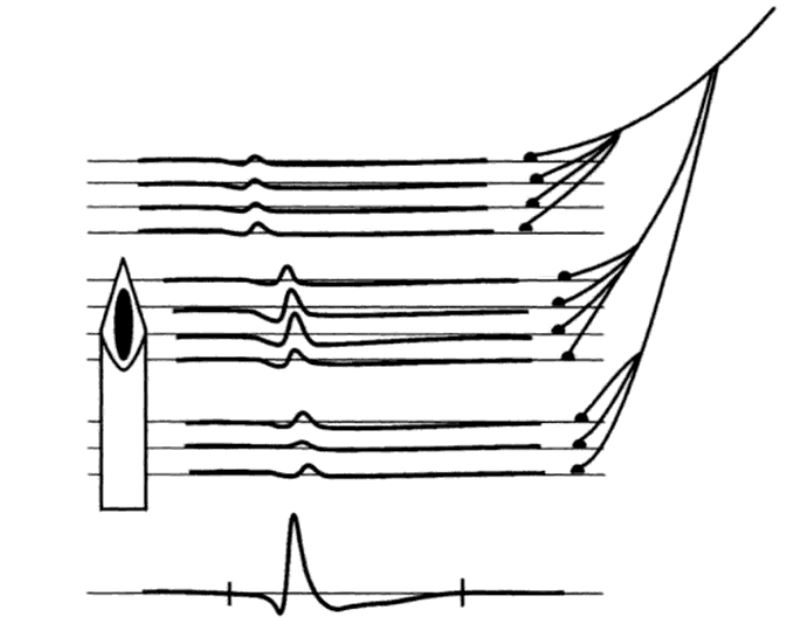
\includegraphics[width = 0.8\textwidth]{img/Merletti2004_EMG.JPG}
\caption[Eletrodo em Forma de Agulha Para Eletromiografia de Profundidade]{Unidade motora do potencial de ação detectada por um eletrodo em forma de agulha concênctrica. Os potenciais de ação das fibras musculares mais próximas são detectados com maior amplitude que os potenciais das fibras mais distantes. A chegada dos potenciais de ação individuais de cada fibra no eletrodo não é perfeitamente síncrono \cite{merletti2004electromyography}.}
\label{Merletti2004_EMG}
\end{figure}

\subsection{Interface Cérebro-Computador}\label{cap2:sub2.2}

As BCI (Brain-Computer Interface), como são conhecidas as interfaces cérebro-computador, são interfaces que interagem diretamente com o sistema nervoso transformando atividade metabólica cerebral em sinais de controle para dispositivos e aplicações \cite{scherer2007self}, neste caso seriam as intenções de ação de um ser humano. Estes sinais elétricos, conhecidos como sinais eletroencefalográficos, são coletados no escalpo humano e representam flutuações do potencial elétrico correspondentes a variações nas camadas mais externas do córtex cerebral abaixo do escalpo \cite{vidal1973toward}. Assim como a técnica citada em \ref{cap2:sub2.1}, a maior parte das técnicas utilizadas pelas BCI consistem de um estilo de miografia invasiva pois os sinais elétricos são adquiridos diretamente do cérebro do usuário através do escalpo, como foi feito no estudo de \cite{hochberg2012reach}, em que os objetos de estudo deveriam movimentar um braço robótico com um BCI implantado em suas cabeças. 

Dentre as dificuldades que esta técnica enfrenta estão as questões éticas. Para os métodos invasivos de obtenção de dados os estudiosos dizem que esse tipo de tecnologia pode possivelmente levar a perdas neurais significantes e risco de infecção, ainda mais se forem feitas conexões de longo período. E mesmo para os métodos não invasivos, como o electroencefalográfico (EEG) \cite{daly2009feasibility}, para BCI existem questionamentos quanto a invasão de privacidade, já que se torna possível o uso da tecnologia para obtenção de dados sigilosos do usuário sem a sua aprovação \cite{wolpaw2006bci}. Por outro lado o uso da BCI é extenso quando se trata da gama de usuários que podem utilizá-la. Os usuários que desfrutam da BCI podem ser divididos em três grupos, (i) aqueles que não possuem nenhum tipo de controle neuromuscular (incluindo movimento dos olhos), (ii) os que possuem uma capacidade limitada de controle neuromuscular e (iii) os que ainda possuem uma quantidade considerável de controle neuromuscular (como a fala e  controle da mão). Assim pode-se entender que o uso de BCI pelos usuários está mais ligado a extensão da disfunção corporal que a origem da disfunção \cite{wolpaw2006bci}.

\begin{figure}[H]
\centering
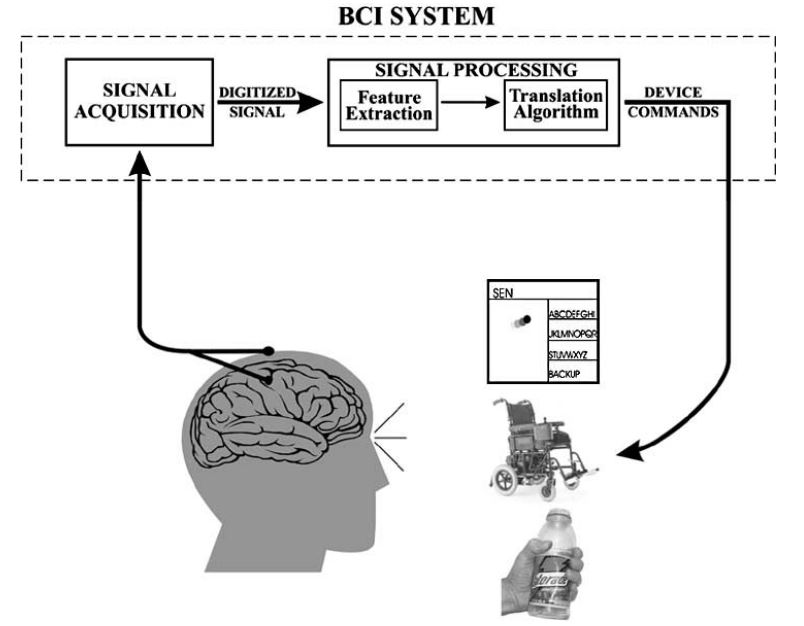
\includegraphics[width = 0.8\textwidth]{img/Schalk2004_BCI.JPG}
\caption[Design Básico de Operação para Qualquer Sistema BCI]{Design básico de operação de qualquer sistema BCI. Sinais que são adiquiridos do cérebro por eletrodos no escalpo, no córtex cerebral ou dentro do cérebro, são processados para extrair aspectos específicos (como amplitudes de potenciais reativos ou ritmos do cortex sensomotor, padrões reativos de neurônios corticais) que refletem a intenção do usuário. Características são traduzidas em comandos que operam um dispositivo (isto é, um simples programa de processamento de palavras, uma cadeira elétrica ou uma prótese neural) \cite{schalk2004bci2000}.}
\label{Schalk2004_BCI}
\end{figure}

\subsection{Eletromiografia de superfície}\label{cap2:sub2.3}

Se um par de eletrodos é colocado na pele de um usuário, sobre o seu músculo, e este é ativado voluntariamente, é possível obter um sinal elétrico entre os eletrodos \cite{merletti2001surface}. Portanto a técnica de eletromiografia de superfície (sEMG) é considerada uma técnica de miografia não invasiva. Desde os anos 1960 a sEMG (\textit{surface electromyography}) é utilizada para controlar manipuladores robóticos em forma de mão com um grau de liberdade já que, como uma técnica não invasiva, dispensa cirurgias ou internação, e mesmo após anos de uma amputação os sinais continuam claros e mais puros que os obtidos diretamente do cérebro, através de métodos não invasivos \cite{castellini2014proceedings}. Apesar de extensamente estudada, a sEMG ainda apresenta limitações no que tange a sua aplicação para membros biônicos como, por exemplo, falta de robustez nas medições, que eram alteradas por eventos fisiológicos dos pacientes, como o suor na pele e a fadiga do músculo \cite{castellini2014proceedings}.

\begin{figure}[H]
\centering
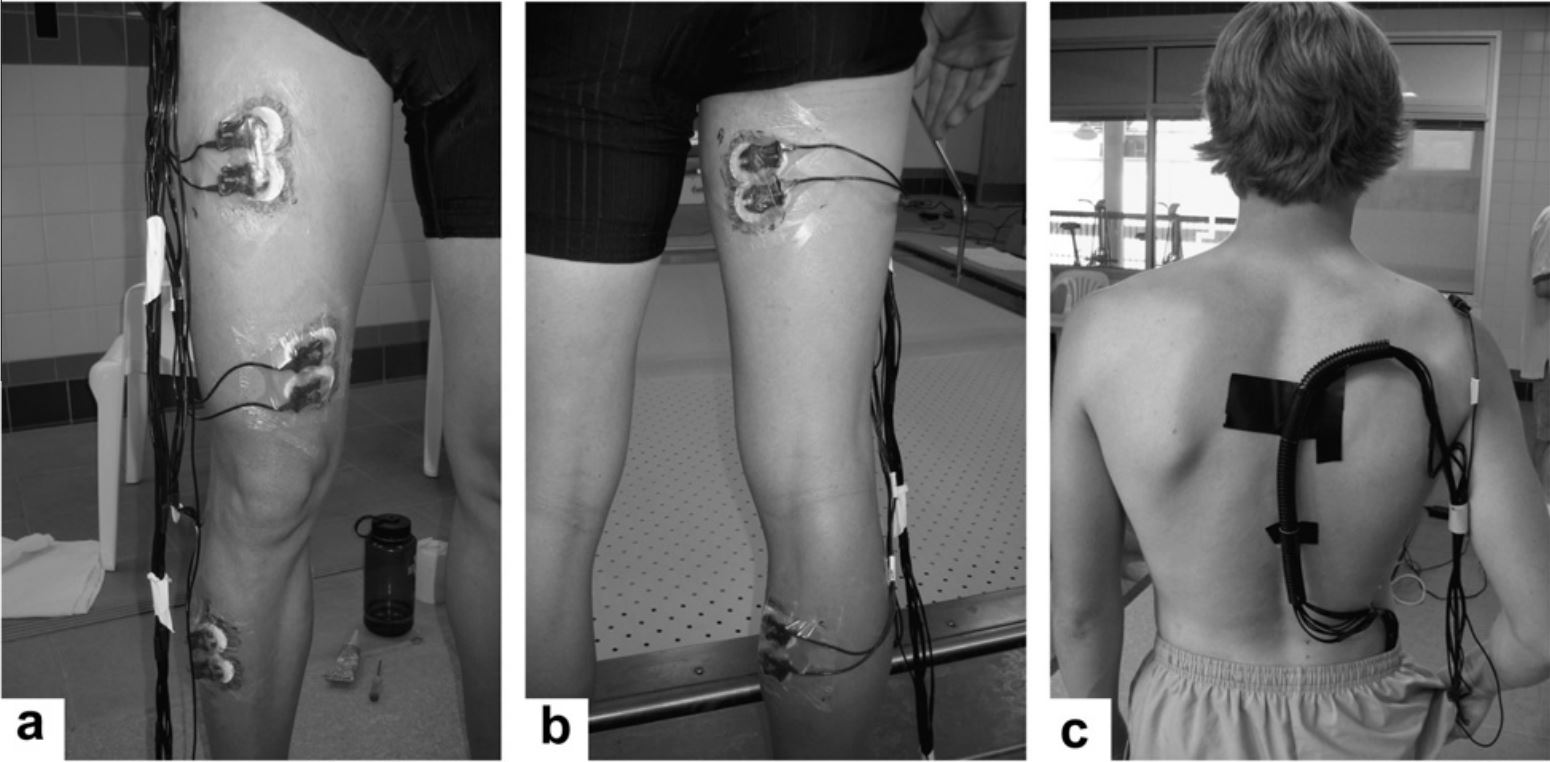
\includegraphics[width = 0.8\textwidth]{img/Silvers2009_sEMG.JPG}
\caption[Montagem Para Testes de Contração Muscular Submerso em Água]{Os fios foram guidaos ao longo da lateral da perna direita (a,b) até a área lombar, onde foram unidos por um tubo plástico, passando pela espinha torácica (c)\cite{silvers2011comparison}.}
\label{Silvers2009_sEMG}
\end{figure}
		

\subsection{Mecanomiografia}\label{cap2:sub2.4}

Com o avanço das técnicas não invasivas surgiu um tipo de tecnologia que remete a observações feitas há mais de trezentos anos, as quais possuiam limitações que não permitiram o seu desenvolvimento tecnológico na época. A tecnologia em questão é a mecanomiografia (MMG), uma técnica que registra as vibrações ou sons produzidos pelo músculo esquelético ao se contrair \cite{vaz1999mecanomiografia} \cite{shinohara1997mechanomyography}.

A MMG se baseia no fato de que as vibrações do músculo ao se contrair são causadas pela contração tetânica incompleta das unidades motoras, portanto é uma técnica não-invasiva, e algumas aplicações deste tipo de miografia incluem o estudo do padrão da fadiga muscular, controle motor, propriedades musculares, frequência da ressonância do músculo e estimativa da força do músculo \cite{shin2016fatigue}. Uma das desvantagens mostradas pelas pequisas sobre esta técnica é a relação entre a taxa de disparo de uma unidade motora e a frequência de informações no sinal da MMG \cite{shin2016fatigue}\cite{shinohara2006mechanomyography}, assim como a dificuldade na montagem para alguns procedimentos o que a torna inviável para algumas rotinas clínicas \cite{hemmerling2004phonomyography}. 

A MMG pode ser um método melhor para aquisição de dados pois possui menos impedimentos, erros no sinal adquirido e processamento de sinal que a sEMG \cite{al2014novel}. Como a amplitude do sinal na MMG é relacionada com a produção de força no músculo, então até uma pequena alteração na força já demonstra alteração no sinal adquirido, enquanto pequenas mudanças de força não são refletidas no sinal adquirido da sEMG \cite{sarillee2014non}.

\begin{figure}[H]
\centering
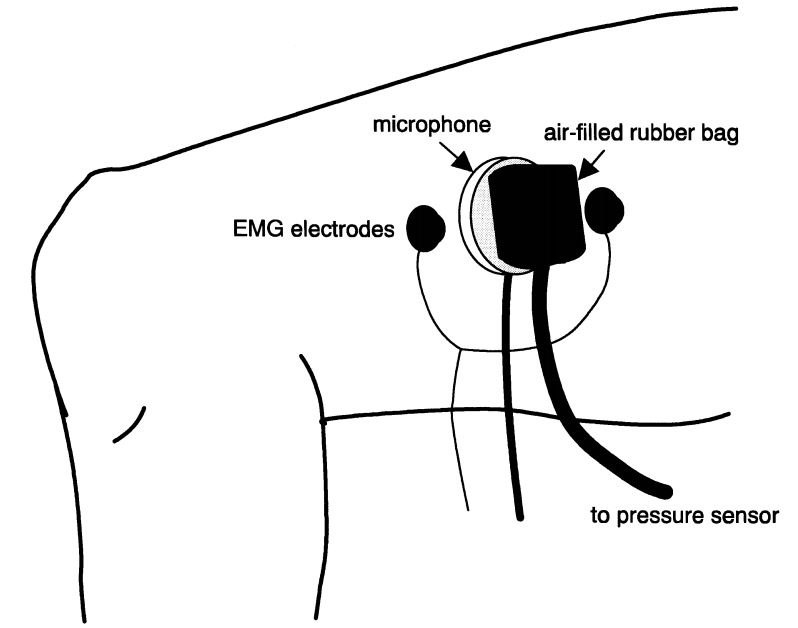
\includegraphics[width = 0.8\textwidth]{img/Shinohara1997_MMG.JPG}
\caption[Diagrama da Montagem Para Medição da EMG, MMG e Pressão]{Diagrama da montagem para a medição da eletromiografia (EMG), a mecanomiografia (MMG), e pressão\cite{shinohara1997mechanomyography}.}
\label{Shinohara1997_MMG}
\end{figure}
 
\subsection{Miografia de Força}\label{cap2:sub2.5}

Tentando melhorar a captação de sinais dos movimentos voluntários, surgem novas técnicas utilizando tecnologias diferentes para superar as barreiras impostas pelos outros métodos já citados. Um novo método que começou a ser desenvolvido recentemente é a miografia de força (FMG). Este método é baseado na medidas dos padrões de resposta mecânica, a força do músculo é medida utilizando um conjunto de sensores de força sobre o músculo para gerar um mapa topográfico de força da atividade muscular e assim decodificar os comandos motores \cite{rasouli2015stable}. Uma aplicação da tecnologia foi estudada em \cite{ravindra2014comparative}, onde foram testadas 3 tecnologias de miografia não invasivas, neste estudo foram analisadas as capacidades de se controlar uma mão prostética de múltiplos dedos. No estudo de \cite{ravindra2014comparative} pode-se notar que a tecnologia da FMG se sobrepõe a EMG pois ela continua com as leituras estáveis mesmo após algum tempo, que é uma das desvantagens da EMG, a fadiga do músculo.

\begin{figure}[H]
\centering
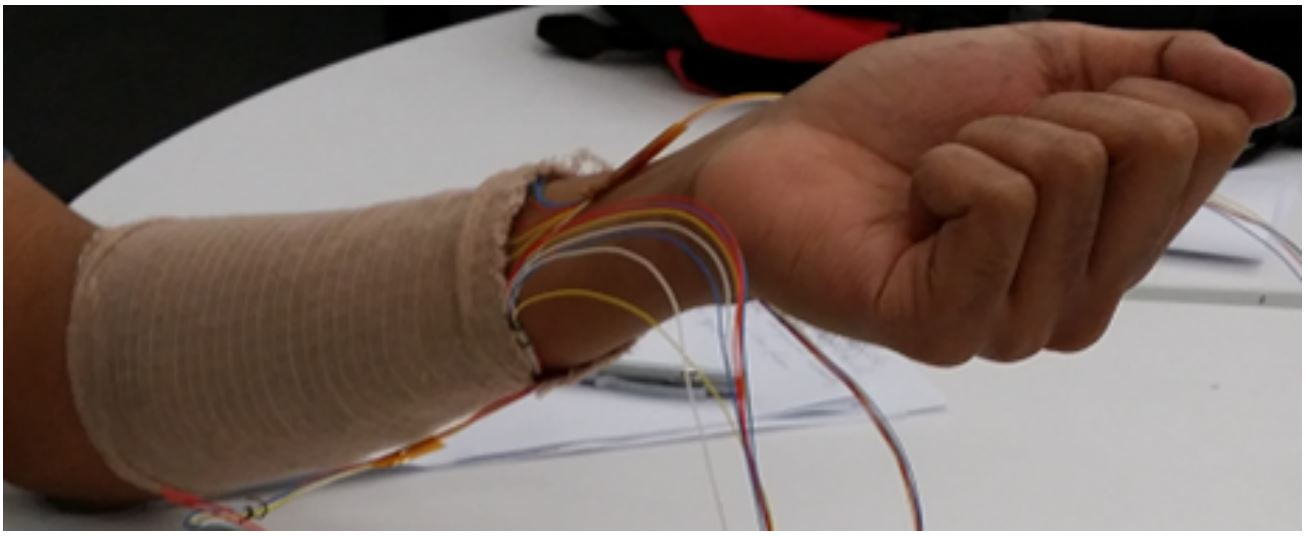
\includegraphics[width = 0.8\textwidth]{img/Rasouli2015_FMG2.JPG}
\caption[Montagem Experimental da FMG]{Montagem experimental de \cite{rasouli2015stable} para obtenção dos sinais de força pela FMG.}
\label{Rasouli2015_FMG}
\end{figure}

\section{Cinemática da Mão}

\subsection{Anatomia da Mão}
\label{anatomia_mao}
A mão humana, como já dito, é uma ferramenta dotada de grande riqueza funcional graças à sua função principal: a preensão. O ser humano é o único capaz de realizar tal ação em um grau de perfeição, e isto se dá ao fato de apresentar um polegar opositor. A mão representa a \textit{"extremidade realizadora"} do membro superior e é altamente articulada \cite{kapandji1971physiology}. 

Para modelar a articulação dos dedos é necessário definir a estrutura cinemática da mão. A mão possui 4 tipos básicos de ossos: metacarpos; falanges próximas; falanges médias; e falanges distais. E possui 4 tipo de juntas básicas: interfalangial distal (DIP); interfalangial próxima (PIP); metacarpofalangial (MP); e interfalangial (IP). A anatomia dos ossos e juntos da mão humana é mostrada na figura \ref{Lee_Kunis_Mao}, na mesma figura os dedos são referenciados como sendo: I - Polegar; II - Indicador; III - Médio; IV - Anelar; e V - Mínimo. As juntas são responsáveis por dar a mão os graus de liberdade (GL), e existem 4 tipos de juntas neste caso: torção, flexão, diretiva e esférica. As juntas de torção e flexão (com um GL) representam a pronação do antebraço e os movimentos de joelho ou ombro, respectivamente. A junta diretiva (com dois GL) permite a flexão em duas direções distintas. A junta esférica (com três GL) permite movimentos diretivos e de torção ao mesmo tempo \cite{lee1995model}. Portanto para os dedos indicador, médio, anelar e mínimo pode ser usada a mesma modelagem cinemática, onde são definidos 4 GL, e não se considera a junta da palma da mão, a qual adicionaria mais um grau de liberdade. E o polegar apresenta 5 GL\cite{lee1995model}.

\begin{figure}[H]
\centering
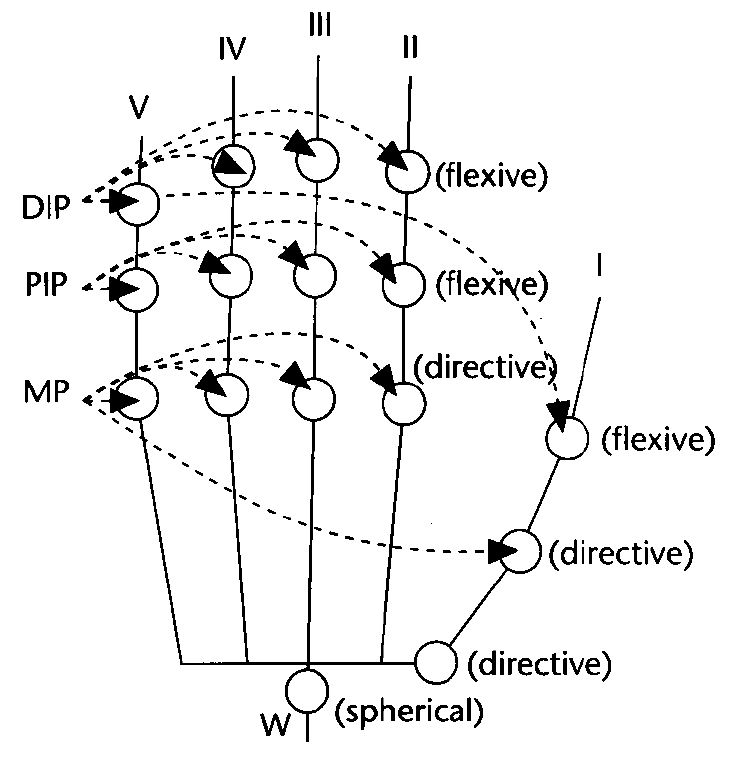
\includegraphics[width = 0.8\textwidth]{img/Lee_Kunis_Mao.JPG}
\caption[O esqueleto da mão observado pelo lado da palma]{Esqueleto da Mão \cite{lee1995model}.}
\label{Lee_Kunis_Mao}
\end{figure}

Existem trabalhos que abordam diferentes modelos para a mão humana.  \cite{bray2005stochastic} propõe um modelo com 26 GL, \cite{kuch1994human} descreve um modelo com 23 GL, \cite{chalfoun2004muscle} e \cite{renault2001dynamic} propõem um modelo com 20 GL, enquanto \cite{du20073d} traz um modelo de 26 GL. No trabalho de \cite{cobos2008efficient} é utilizado um modelo de 24 GL contra dois modelos de 9 e 6 GL, afim de discutir os erros de posição que a diferença de GL proporciona. Os modelos apresentam diferentes GL devido as restrições, impedindo que a mão não possa fazer gestos arbitrários. Por exemplo o dedo mínimo não consegue ser dobrado sem que se dobre o dedo anelar \cite{lin2000modeling}.

Segundo \cite{lin2000modeling} as restrições da mão podem ser divididas em três tipos. Restrições do tipo 1 são referentes aos limites dos movimentos dos dedos como resultado da anatomia da mão. Restrições do tipo 2 são limites impostos nas juntas quando em movimento. Restrições do tipo 3 acontecem devido a performance natural da mão, e ainda não foram amplamente estudadas.

\begin{figure}[H]
\centering
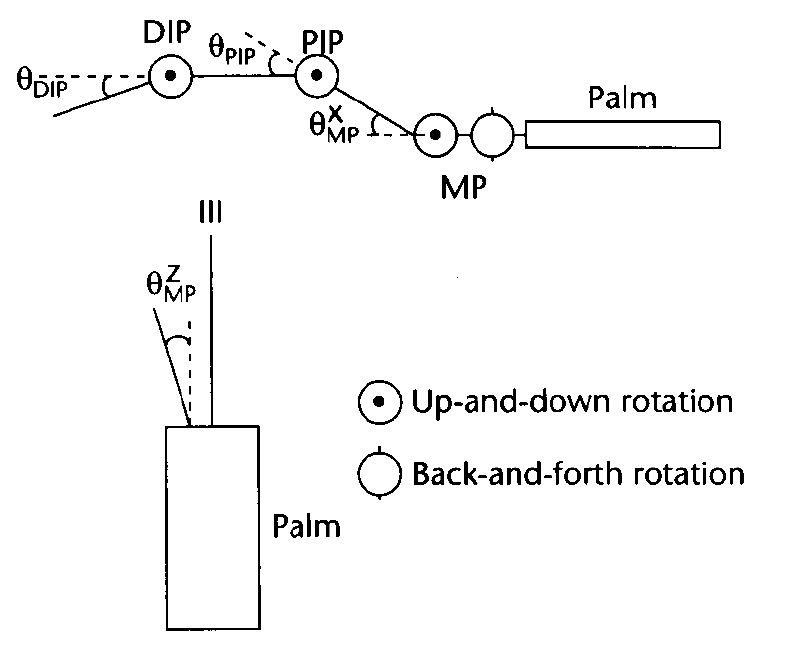
\includegraphics[width = 0.8\textwidth]{img/Lee_Dedo.JPG}
\caption[As juntas de um dedo representadas com seus ângulos]{Mecanismos da mão representados por símbolos de juntas \cite{lee1995model}.}
\label{Lee_Dedo}
\end{figure}

\subsubsection{Restrições do Tipo 1}\label{Tipo 1}
Este tipo de restrição está atrelado aos limites de alcance da movimentação dos dedos como um resultado da anatomia da mão. Neste caso para se impor a restrição é necessário levar em conta que não há forças externas atuando sobre o movimento dos dedos. Portanto podemos determinar restrições como:

\begin{align}
0^\circ < \theta_{MP_F} \leq 90^\circ, \\
0^\circ < \theta_{PIP_F} \leq 110^\circ, \\
0^\circ < \theta_{DIP_F} \leq 90^\circ, \\
-15^\circ < \theta_{MP_{AA}} \leq 15^\circ.
\end{align}

onde o subescrito F se aplica para o movimento de flexão e o subescrito AA o movimento de abdução e adução.

Outra restrição usualmente adotada é relativa aos movimentos de abdução e adução do dedo médio, pois neste são quase inexistentes. Da mesma maneira, a junta metacarpofalangial do polegar não apresenta tais movimentos de abdução e adução.

\begin{align}
\theta_{MP_{AA}} = 0^\circ
\end{align}

Os dedos indicador, médio, anelar e mínimo são considerados manipuladores planares, ou seja, das juntas DIP, PIP e IP de cada dedo se movimentam em apenas um plano, já que as juntas DIP e PIP possuem um grau de liberdade \cite{lin2000modeling}.

\subsubsection{Restrições do Tipo 2}\label{sssec:Tipo2}
Este tipo de restrição se refere aos limites impostos nas juntas durante a movimentação dos dedos. Estas restrições podem em si serem divididas em outras duas subdivisões, uma relativa ao movimento do dedo consigo mesmo e a outra relativa ao movimento de um dedo em relação a outro.

As relações entre dedos é dada entre juntas de dedos adjacentes, como por exemplo quando a junta MP do dedo indicador é dobrada, a junta MP do dedo médio é forçada a se dobrar também \cite{lin2000modeling}.

A relação entre as juntas de um mesmo dedo é frequentemente representada pela restrição em que quando a junta DIP é dobrada, a junta PIP correspondente deve ser dobrada também \cite{lin2000modeling}\cite{lee1995model}. Esta restrição pode ser aproximada de tal forma que:

\begin{align}
\theta_{DIP} = \frac{2}{3} \theta_{PIP} \label{relacao_dip_pip}
\end{align}

\subsubsection{Restrições do Tipo 3}\label{Tipo 3}
Segundo \cite{lin2000modeling} estas restrições são impostas pela natureza dos movimentos da mão humana e portanto são mais difíceis de se detectar e quantificar. As restrições do tipo 3 se diferem das restrições do tipo 2 pelo fato de não estarem atreladas as limitações da anatomia da mão humana, mas são um resultado de movimentos naturais. Por exemplo, a maneira mais natural de se fechar a mão é flexionando todos os dedos quase que ao mesmo tempo, ao invés de curvar um dedo de cada vez. Este tipo de restrição não pode ser representado por uma equação já que difere de pessoa para pessoa e ao mesmo tempo é similar para muitos.

\subsection{Propriedades e Modelos dos Músculos}\label{propriedades_musculo}
A partir do modelo cinemático da mão pode-se estabelecer a relação entre o ângulo formado pelas juntas dos dedos e a posição final da ponta dos dedos. Para que o dedo assuma tal posição, de forma direta, se faz necessário determinar como os músculos dos membros superiores, majoritariamente mão e antebraço, funcionam com o objetivo de movimentar o dedo de tal forma que a sua ponta atinja o ponto final.

\subsubsection{Anatomia Muscular}
Os músculos podem ser considerados um conjuntos de fibras igualmente longas, chamadas de células, em paralelo. As fibras do músculo estão orientadas em direção do tendão ou em um ângulo agudo em relação ao tendão, como demonstrado na figura \ref{fibras}, sendo $\alpha$ o ângulo agudo. Este ângulo $\alpha$ representa a orientação das fibras em relação ao eixo de ação do tendão. Pode-se notar que conforme o tendão se estica, $\alpha$ aumenta e assim sendo as fibras contraem em uma direção que não é colinear com a direção em que o tendão estica \cite{zajac1989muscle}.

\begin{figure}[H]
\centering
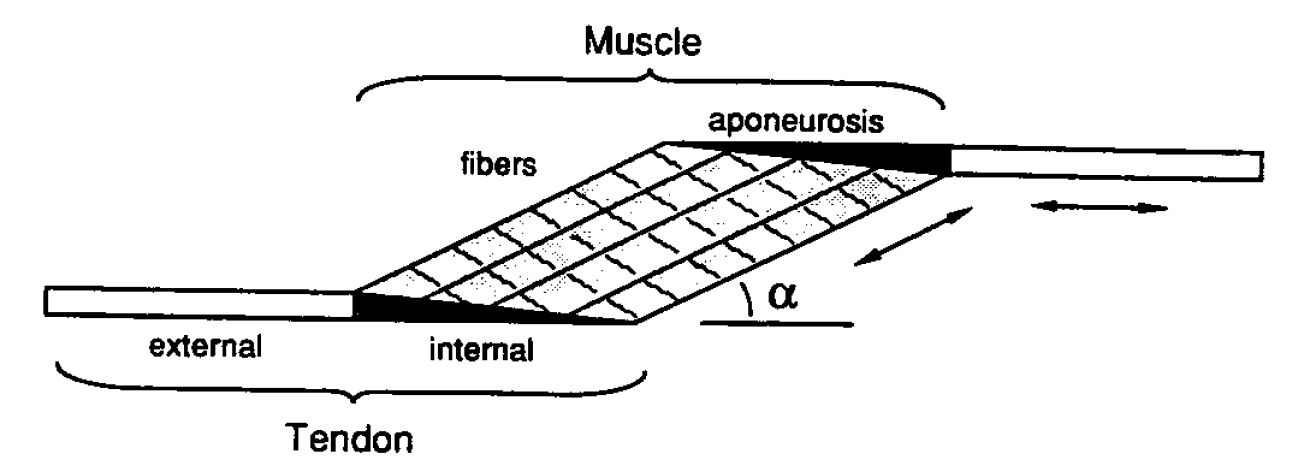
\includegraphics[width = 0.8\textwidth]{img/Zajac1989_FibrasMusculares.JPG}
\caption[Representação das Fibras Musculares]{Relação entre as fibras musculares e o tendão em um músculo penado \cite{zajac1989muscle}}
\label{fibras}
\end{figure}

Uma fibra muscular de tamanho $L_m$ pode ser considerada um conjunto de sarcômeros de mesmo tamanho $L_s$, os quais são estimulados simultaneamente para produzir a força F, demonstrados na figura \ref{sarcomeros}. Os sarcômeros, por sua vez, são constítuidos de filamentos finos (actina) e espessos (miosina) que deslizam entre si para produzir o movimento de contração do músculo.

\begin{figure}[H]
\centering
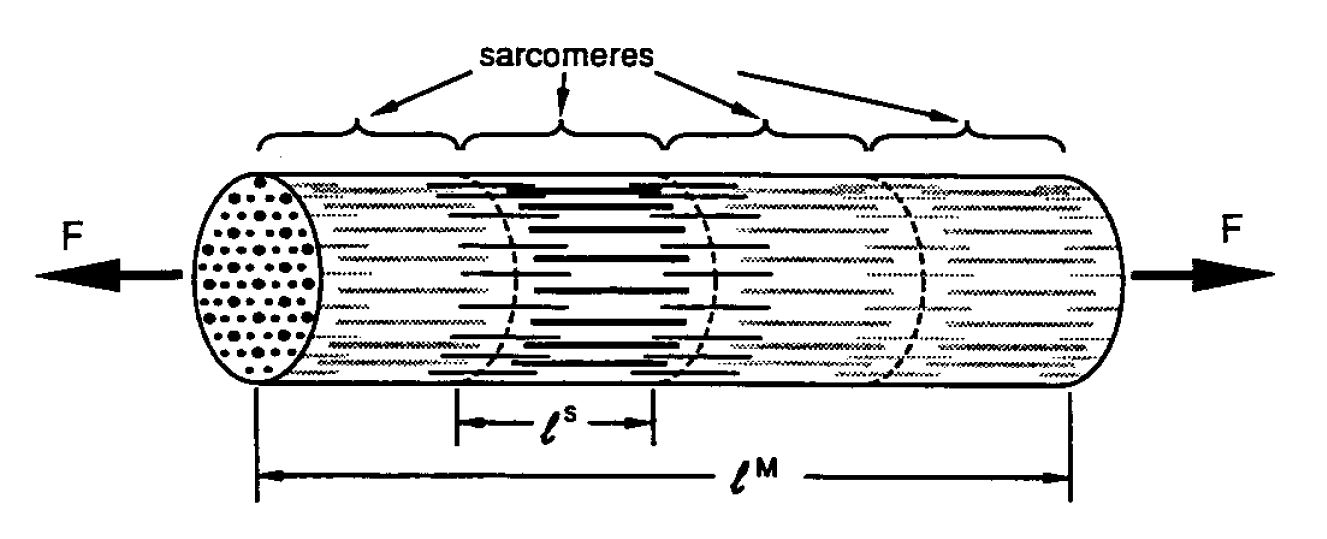
\includegraphics[width = 0.8\textwidth]{img/Zajac1989_Sarcomeros.JPG}
\caption[Representação dos Sarcômeros]{Representação da fibra muscular e a estrutura de sarcômeros \cite{zajac1989muscle}}
\label{sarcomeros}
\end{figure}

Uma unidade motora é definida como um axônio e um conjunto de fibras musculares enervadas por este axônio e seus ramos \cite{burke2011motor}. Um músculo pode ser representado por \textit{n} unidades motoras sendo controladas por \textit{n} axônios originados no sistema nervoso central, cada um deles com o seu controle $u_i(t)$. A força $F^i_m$, originada em uma unidade motora, é proveniente das fibras musculares que agem em conjunto para desenvolvê-la, como é representado na figura \ref{unidademotora}.  Pode-se dizer, então, que a soma das forças $F^i_m$ produzem a força muscular líquida $F_m$.

\begin{figure}[H]
\centering
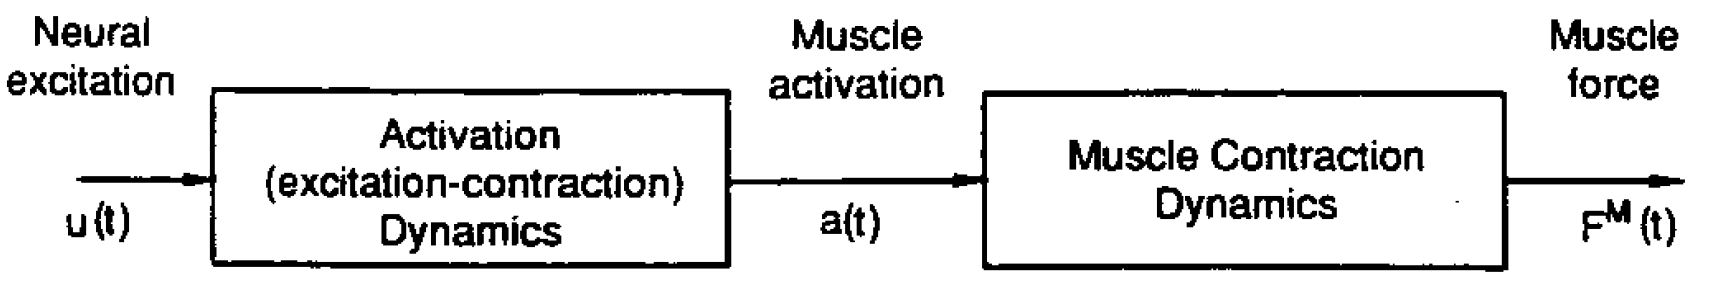
\includegraphics[width = 0.8\textwidth]{img/Zajac1989_UnidadeMotora.JPG}
\caption[Representação da Produção de Força em uma Unidade Motora]{Dinâmimca do tecido muscular\cite{zajac1989muscle}}
\label{unidademotora}
\end{figure}

A dinânimca contracional do músculo pode ser dividida entre: dinâmica de ativação e dinâmica de contração. A dinâmica de ativação diz respeito a transformação de estímulos neurais em ativação dos elementos contráteis. A dinâmica de contração diz respeito a transformação de ativação em força muscular. Existem duas propriedades que discutem a dinâmica de contração: a propriedade de força-comprimento, que diz respeito a capacidade do tecido muscular em gerar força enquanto se alonga, e a propriedade de força-velocidade, que diz respeito a velocidade em que as fibras finas e espessas se deslocam ao realizar a contração e a quantidade de pontes cruzadas no tecido muscular \cite{zajac1989muscle}.

\subsubsection{Modelo de Hill}
O modelo que descreve uma fibra muscular e é amplamente utilizado na literatura é o modelo de Hill, de 1938 \cite{hill1938heat}. Este modelo parte do pressuposto que as propriedades de contração de um tecido muscular podem ser representadas por uma relação de força-comprimento-velocidade (\textit{flv}) 

A versão simplificada deste modelo é baseada em 3 componentes, presentes na figura \ref{hillmodel}: elemento contrátil (CE), representado por um amortecedor, e mostra a relação entre a intensidade e velocidade da força exercida pelo músculo; elemento elástico em série (SE); e elemento elástico em paralelo (PE). Os elementos SE e PE representam a conexão passiva do tecido, incluindo tendão e fibras musculares não ativas \cite{rosen1999performances}

\begin{figure}[H]
\centering
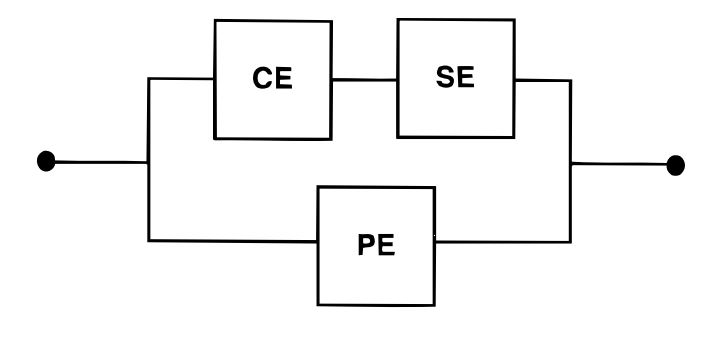
\includegraphics[width = 0.8\textwidth]{img/Rosen1999.JPG}
\caption[Modelo de Hill para uma fibra muscular]{Modelo de Hill para uma fibra muscular. PE = Elemento Elástico Paralelo; CE = Elemento Contrátil; SE = Elemento Elástico em Série \cite{rosen1999performances}.}
\label{hillmodel}
\end{figure}

Mesmo que este modelo seja uma versão simplificada e possua limitações ele é amplamente utilizado devido a facilidade da sua implementação \cite{rosen1999performances}. O modelo de Hill foi aprimorado com o tempo por pesquisadores diferentes, o modelo apresentado no trabalho de \cite{rosen1999performances} tem como base outros trabalhos anteriores como os de Winters (\cite{winters1993effect}, \cite{winters1985task}, \cite{winters1987biomechanical}, \cite{winters1988estimated}). 

Segundo \cite{rosen1999performances} a relação entre força e extensão dos tecidos são definidas pelas seguintes equações:

\begin{align}
F_{SE}=\frac{F_{SEmax}}{e^{SEsh}-1}(e^{SE_{sh}\Delta L_{SE}/\Delta L_{SE_{max}}}-1) \label{forcaSE} \\
F_{SE}=\frac{F_{PEmax}}{e^{PEsh}-1}(e^{PE_{sh}\Delta L_{PE}/\Delta L_{PE_{max}}}-1) \label{forcaPE}
\end{align}

Estas relações representam o comportamento do músculo no esqueleto, como a força exercida pelos componentes se relaciona ao comprimento dos componentes. $F_{SE}, \Delta L_{SE}$ e $F_{PE},\Delta L_{PE}$ são, respectivamente, a força e a extensão de cada componente, e o subescrito \textit{max} denota os valores máximos para o correspondente. $SE_{sh}$ e $PE_{sh}$ são parâmetros em função da forma ("\textit{shape}").

O componente elástico (CE) representa as fibras ativas do músculo e existem duas relações para definí-lo: a relação força-comprimento e a relação força-velocidade. \cite{rosen1999performances} representa a força total gerada por CE como:

\begin{align}
F_{CE} = f_{FV}(V_{CE}) \cdot f_{FL}(L_{CE}) \cdot F_{max} \cdot U \label{forcaCE}
\end{align}

Onde $F_{CE}$ é a força no componente CE, $f_{FV}$ e $f_{FL}$ são funções adimensionais para força-velocidade e força-comprimento, respectivamente. $F_{max}$ é a força máxima em CE, $V_{CE}$ e $L_{CE}$ são, respectivamente, a velocidade de deslocamento e o próprio comprimento de CE, $U$ é o nível normalizado de ativação do componente. O nível de ativação do músculo tem o objetivo de diferenciar movimentos suaves de movimentos fortes. As funções $f_{fv}$ e $f_{FL}$ são descritas em \ref{funcveloc} e \ref{funcdesloc}

\begin{align}
f_{FV} = \frac{0,1433}{0,01074+ e^{-1,409sinh(3,2V_{CE}/V_{max}+1,6)}} \label{funcveloc} \\
f_{Fl} = e^{(-0,5((L_{CE}/L_0-1,05)/0,19)^2} \label{funcdesloc}
\end{align}


Onde $L_{CE}$ e $L_0$ são o comprimento do músculo e o comprimento do músculo relaxado, respectivamente. $V_{max}$ e $V_{0}$ são a velocidade máxima do músculo e a velocidade específica para a ativação do músculo no momento do movimento desejado, respectivamente.

Com as equações de \ref{forcaSE} até \ref{funcdesloc} é possível prever a força que será realizada pelo músculo com o uso apenas de dados anatômicos do ser humano em questão, o que torna o estudo escalável.



%------------------------------------------------------------------------------



% ---------------------------------------------------------------
%                                   CAPÍTULO 3
% ---------------------------------------------------------------
%\clearpage


\selectlanguage{Brazilian}

\chapter{MATERIAIS E MÉTODOS}\label{cap3}

\section{Modelagem Cinemática da Mão}

\subsection{Cinemática Direta da Mão}
\label{cinematica_direta_mao}
A partir do conjunto de restrições apresentado em \ref{anatomia_mao}, passamos a ter um modelo com 15 GL \cite{lin2000modeling}. E pode-se obter a cinemática direta, com o objetivo de calcular a posição e orientação da ponta do dedo a partir dos ângulos das juntas. A cinemática da mão pode ser subdividida em dois conjuntos: cinemática do polegar e cinemática dos dedos restantes. A cinemática direta é obtida por meio das matrizes de parâmetros de Denavit-Hartenberg (DH) \cite{hartenberg1964kinematic}, estas são frequentemente utilizadas em modelagem de braços robóticos \cite{cobos2008efficient}.

A transformação de Denavit-Hartenberg é a mais utilizada para representação cinemática de juntas concatenadas. Ela é baseada na transformação entre juntas sucessivas, e estas expressas por 3 parâmetros fixos e um variável (dependente do tipo de junta) \cite{newman2000calibration}. Os parâmetros de DH que, portanto, descrevem as juntas são: $a_i$, que representa o comprimento da conexão entre duas juntas; $\alpha_i$, que representa a rotação entre uma junta e o sua sucessiva dado o eixo de ação da junta; $d_i$, que representa \textit{offset} da junta, ou seja, a distância de uma junta até a próxima ao longo do eixo de ação de i; e $\theta_i$, que representa o ângulo de uma junta, ou seja, a rotação de uma junta em relação a próxima sobre o eixo de ação de i. Os parâmetros $a_i$ e $\alpha_i$ são os parâmetros que definem a posição relativa de duas juntas no espaço, enquanto os parâmetros $d_i$ e $\theta_i$ são os parâmetros variáveis, que definem o tipo da junta\cite{corke2007simple}.

A representação de DH é feita, portanto, por matrizes de transformação, as quais relacionam as coordenadas de uma junta i em relação a base do sistema por meio de:

\begin{align}
\label{RepDH}
A_i(\theta_i,d_i,a_i,\alpha_i) = R_z(\theta_i)T_z(d_i)T_x(a_i)R_x(\alpha_i)
\end{align}

Onde $R_k$ representa a rotação em torno do eixo \textit{k} e $T_k$ representa a translação ao longo do eixo \textit{k}. Para um manipulador com n juntas pode-se expressar a transformação total do manipulador em função das transformações de suas juntas individuais \cite{corke2007simple}.

\begin{align}
\label{TransDH}
T^{0}_n = A^{0}_1 A^{1}_2 ... A^{n-1}_n
\end{align}

\cite{craig2005introduction} expressou um conjunto de juntas genéricas para exemplificar o conceito da obtenção dos parâmetros de DH

\begin{figure}[H]
\centering
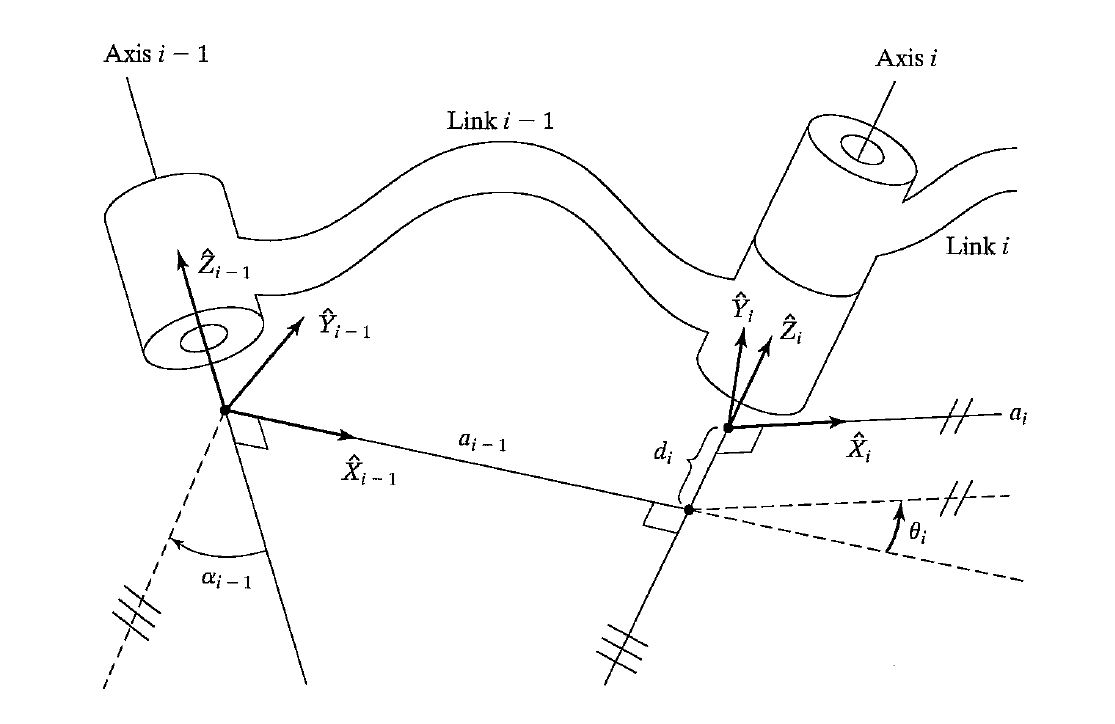
\includegraphics[width = 0.8\textwidth]{img/Craig_DHLinks.JPG}
\caption[Representação das Juntas para Obtenção dos Parâmetros de DH]{Juntas Genéricas para DH \cite{craig2005introduction}}
\label{Rocha2011}
\end{figure}

\subsubsection{Dedos Indicador, Médio, Anelar e Mínimo}
Sem considerar o osso metacarpo, que é o osso que faz a ligação dos dedos com a palma, os dedos indicador, médio, anelar e mínimo possuem 3 juntas: MP, PIP e DIP, e 3 ossos: próximo, médio e distal. Como definidas por \cite{lee1995model} as duas juntas flexivas mais a junta diretiva formam 4 GL. A tabela \ref{DHResto} mostra os parâmetros da matriz de DH e a figura \ref{JuntasResto} mostra a configuração das juntas para determinação dos parâmetros de DH.

\begin{table}[H]
\centering
\caption{Parâmetros da Matriz DH - Indicador,Médio,Anelar e Mínimo}
\label{DHResto}
\begin{tabular}{|c|c|c|c|c|}
	\hline
    Juntas & a & $\alpha$ & d & $\theta$ \\ \hline
    1 & 0 & $0^\circ$ & 0 & $\theta_1$ \\ \hline
    2 & 0 & $-90^\circ$ & 0 & $\theta_2$ \\ \hline
    3 & $l_1$ & $0^\circ$ & 0 & $\theta_3$ \\ \hline
    4 & $l_2$ & $0^\circ$ & 0 & $\theta_4$ \\ \hline
    5 & $l_3$ & $0^\circ$ & 0 & $\theta_5$ \\
	\hline
\end{tabular}
\end{table}

\begin{figure}[H]
\centering
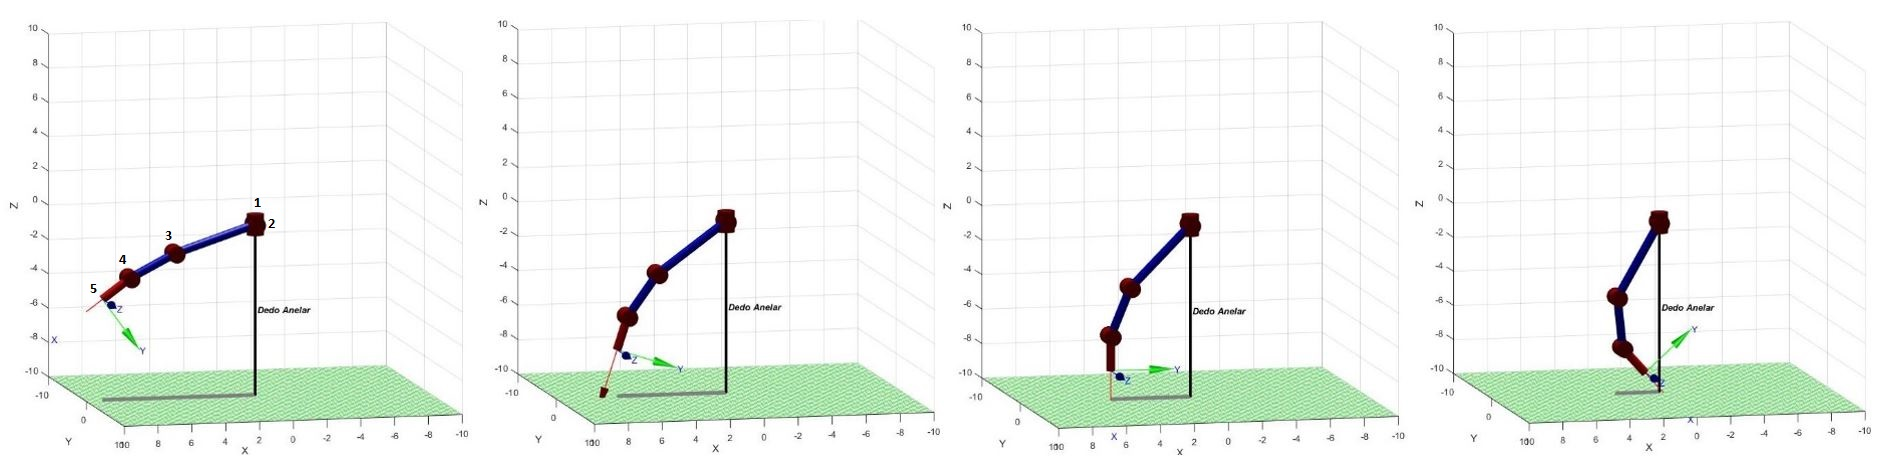
\includegraphics[width = 1\textwidth]{img/Anelar.JPG}
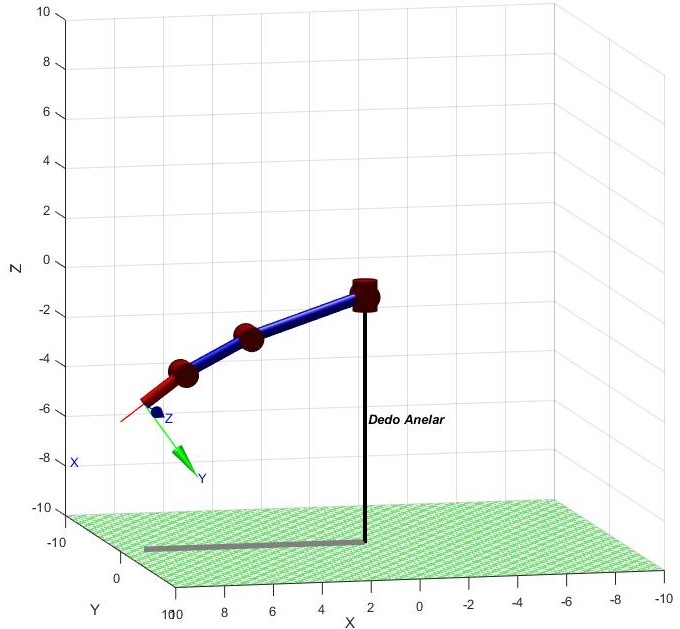
\includegraphics[width = 0.65\textwidth]{img/Anelar1.JPG}
\caption[Representação do dedo anelar como um manipulador robótico]{Representação do dedo anelar como um manipulador robótico utilizando o toolbox do \textit{MATLAB} \cite{corke1996robotics}}
\label{JuntasResto}
\end{figure}



\subsubsection{Dedo Polegar}
O polegar possui 3 juntas, sendo duas diretivas e uma flexiva, configurando 5 GL \cite{lee1995model}, e 3 ossos. A tabela \ref{DHPolegar} mostra os parâmetros da matriz de DH e a figura \ref{JuntasPolegar} mostra a configuração das juntas para determinação dos parâmetros de DH. A configuração para a construção do polegar prevê \textit{offsets} para as rotações de coordenadas das juntas, como na junta 4 e 5.

\begin{table}[H]
\centering
\caption{Parâmetros da Matriz DH - Polegar}
\label{DHPolegar}
\begin{tabular}{|c|c|c|c|c|}
	\hline
    Juntas & a & $\alpha$ & d & $\theta$ \\ \hline
    1 & 0 & $0^\circ$ & 0 & $\theta_1$ \\ \hline
    2 & 0 & $90^\circ$ & 0 & $\theta_2$ \\ \hline
    3 & 0 & $0^\circ$ & $l_1$ & $\theta_3$ \\ \hline
    4 & 0 & $90^\circ$ & 0 & $\theta_4 + \frac{\pi}{2}$  \\ \hline
    5 & -$l_2$ & $0^\circ$ & 0 & $\theta_5 - \frac{\pi}{2}$ \\ \hline
    6 & -$l_3$ & $0^\circ$ & 0 & $\theta_6$ \\
	\hline
\end{tabular}
\end{table}

\begin{figure}[H]
\centering
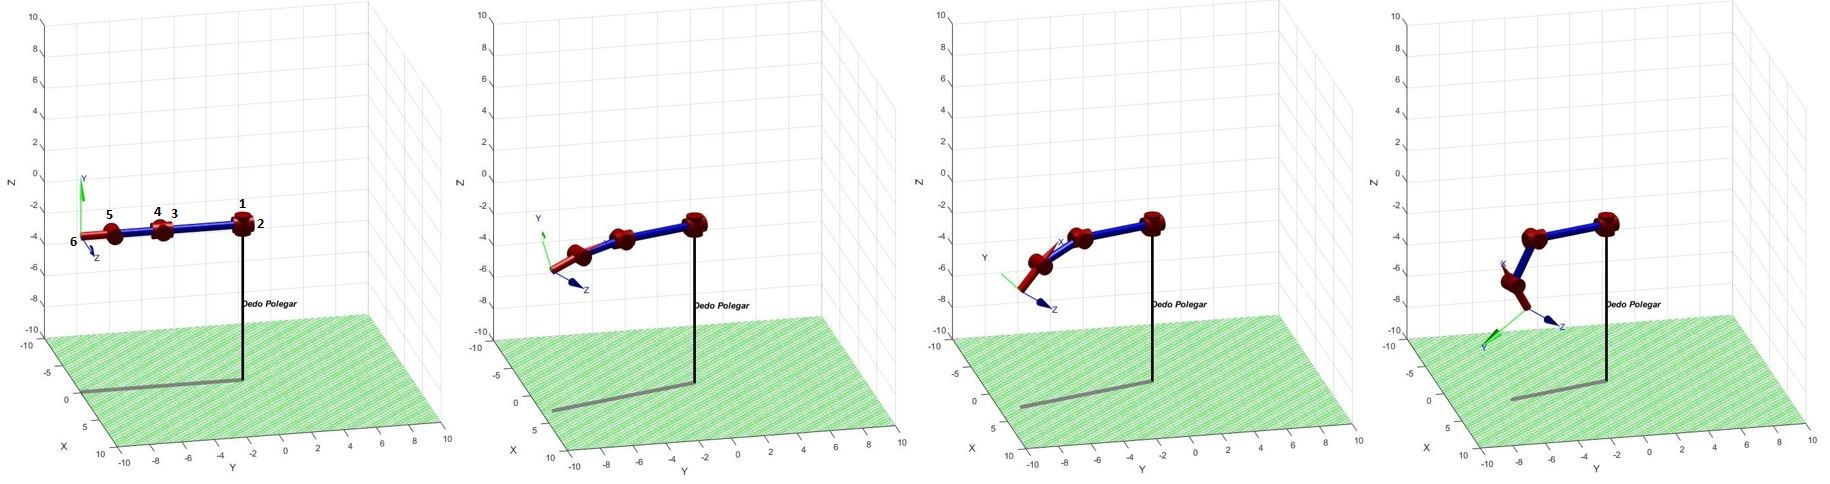
\includegraphics[width = 1\textwidth]{img/Polegar.JPG}
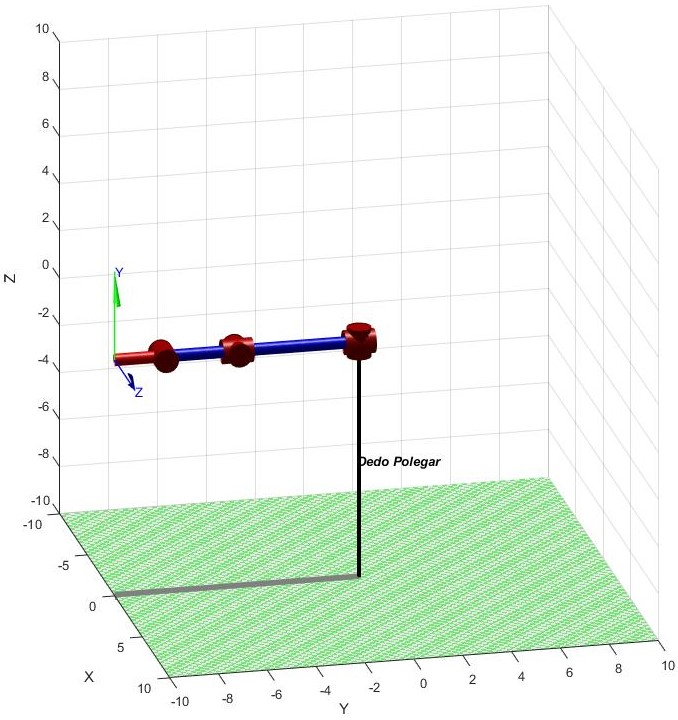
\includegraphics[width = 0.65\textwidth]{img/Polegar1.JPG}
\caption[Representação do dedo polegar como um manipulador robótico]{Representação do dedo polegar como um manipulador robótico utilizando o toolbox do \textit{MATLAB} \cite{corke1996robotics}}
\label{JuntasPolegar}
\end{figure}

\subsection{Simulação da Mão}
Neste projeto a simulação da mão é implementada utilizando uma toolbox do \textit{MATLAB} de código open source do proprietário Peter Corke \cite{corke1996robotics}, a "Robotics Toolbox for MATLAB". Com o uso desta toolbox é necessário implementar as matrizes de DH, que definirão os chamados \textit{Links} e ao unir-los, criando um \textit{SerialLink}, podemos definir as posições espaciais dos dedos utilizando a cinemática direta, ou seja, passando como parâmetros os ângulos de cada junta. Os ângulos de cada junta por sua vez são obtidos do modelo de Hill \cite{hill1938heat} que estão explicados com mais detalhes na seção \ref{modelagem_antebraco}. 

É possível criar uma visão de alto nível de como a modelagem cinemática da mão, e assim sua simulação, interage diretamente com a modelagem dos músculos do antebraço, e portanto o modelo de Hill, como na imagem \ref{IntegracaoAltoNivel}

\begin{figure}[H]
\centering
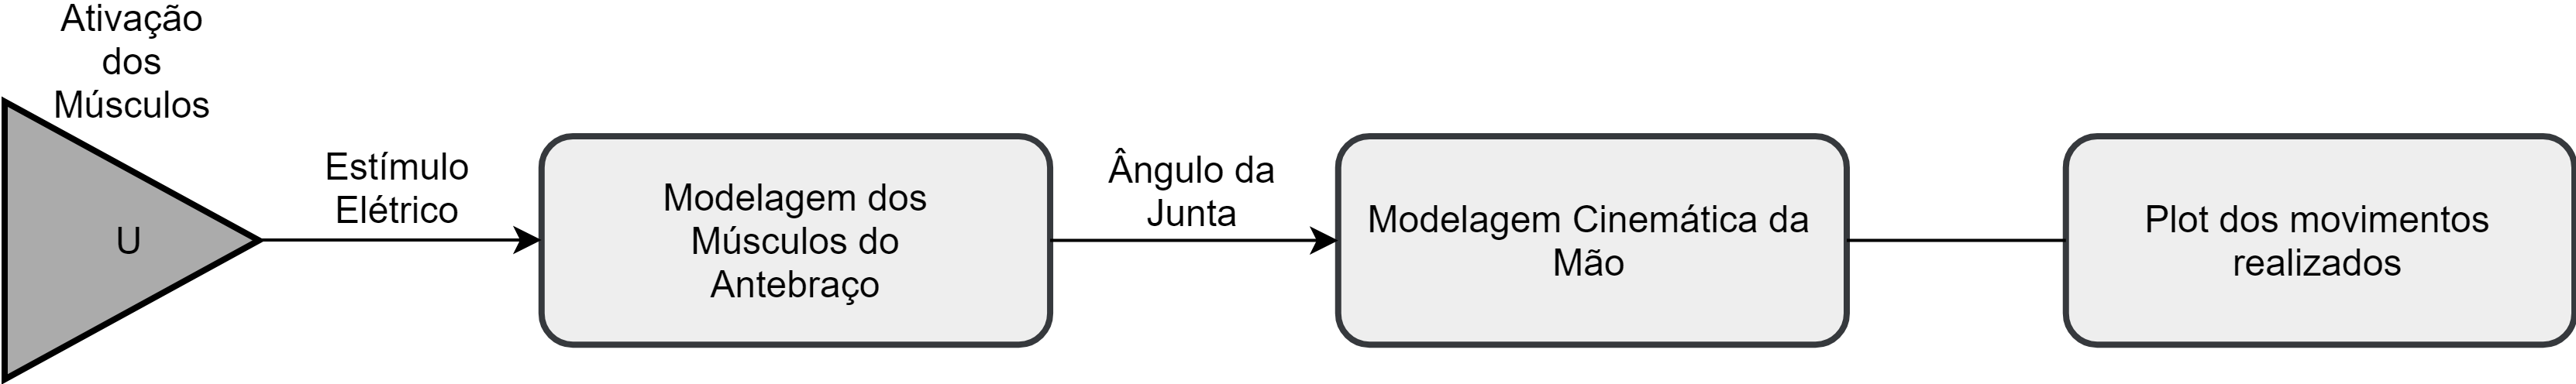
\includegraphics[width = 1\textwidth]{img/integracao_alto_nivel.JPG}
\caption[Integração em alto nível]{Integração em alto nível da modelagem cinemática da mão e da modelagem dos músculos do antebraço}
\label{IntegracaoAltoNivel}
\end{figure}

A implementação dos dedos neste projeto é, como apresentado na cinemática da mão, separada na cinemática do polegar e a cinemática dos demais dedos da mão.Para isto são utilizadas as matrizes de DH obtidas na seção \ref{cinematica_direta_mao}. Os referenciais do plano cartesiano são como os mostrados nas imagens \ref{JuntasResto} e \ref{JuntasPolegar}, tomando como base referencial a primeira junta, a que está na base da falange. Como é um modelo tridimensional, os ângulos das juntas permitem, com base nas restrições da seção \ref{anatomia_mao} descrever a posição dos dedos no espaço.

Dentre os parâmetros de DH, estão os parâmetros dados pela letra l que são, basicamente, as distâncias entre as juntas, e os parâmetros $\theta$ que definem a angulação da junta. Logo, para cada separação podemos definir de antemão os parâmetros estáticos (l) com base em medições realizadas sobre seres humanos comuns.

\begin{table}[H]
\centering
\caption{Parâmetros Definidos Para Indicador,Médio,Anelar e Mínimo}
\label{ParamResto}
\begin{tabular}{|c|c|c|c|c|}
	\hline
    Parâmetro & Valor (cm) & Observação \\ \hline
    $l_1$ & 3 & Comprimento Primeira Falange \\ \hline
    $l_2$ & 2,5 & Comprimento Segunda Falange \\ \hline
    $l_3$ & 2 & Comprimento Terceira Falange \\ \hline
\end{tabular}
\end{table}

\begin{table}[H]
\centering
\caption{Parâmetros Definidos Para o Polegar}
\label{ParamPolegar}
\begin{tabular}{|c|c|c|c|c|}
	\hline
    Parâmetro & Valor (cm) & Observação \\ \hline
    $l_1$ & 5,7 & Comprimento Primeira Falange \\ \hline
    $l_2$ & 4,2 & Comprimento Segunda Falange \\ \hline
    $l_3$ & 2,7 & Comprimento Terceira Falange \\ \hline
\end{tabular}
\end{table}

Uma vez utilizados os parâmetros definidos, é possível utilizando as matrizes de DH obter a posição espacial da ponta de cada dedo, com valores específicos em x,y e z para cada junta também.

\section{Modelagem dos Músculos do Antebraço}
\label{modelagem_antebraco}
Para simular o comportamento dos dedos, como descrito na imagem \ref{IntegracaoAltoNivel}, é necessário que sejam determinados os ângulos das juntas. Estes ângulos são determinados a partir da força produzida pelos músculos como é descrito no modelo de Hill na seção \ref{propriedades_musculo}. Para este projeto usa-se um modelo mais simplificado da relação $flv$ do que as relações descritas por \cite{rosen1999performances}, este modelo aproxima-se mais do modelo descrito por \cite{zajac1989muscle} e \cite{durfee1994estimation} em que o elemento SE pode ser desconsiderado assumindo ser infinitamente rígido, para fins de simplificação, já que a maior parte da força é gerada nos elementos CE e PE. Ao definir as curvas utilizadas no modelo podemos fazer de forma normalizada para que as variações nas medidas possam ser consideradas como ganhos simples.Para que haja adequação dos valores foram utilizados parâmetros encontrados em \cite{lemay1996dynamic}, os quais serão utilizados para determinar os valores dos ângulos das juntas.

\subsection{Músculos Utilizados}
É preciso determinar quais músculos serão tratados no problema, sabendo que cada músculo é responsável pelo movimento de uma, ou mais falanges. A partir da cinemática da mão proposta neste projeto 3 falanges serão movimentadas, as falanges próximas, as falanges médias e as falanges distais, sendo cada uma delas atrelada a uma junta, MP, PIP e DIP. Como simplificação do projeto é modelado que o movimento de avanço e recuo é realizado por músculos diferentes, apesar de agirem sobre a mesma falange e junta. 

Como descrito na restrição tipo 2 da seção \ref{anatomia_mao} a movimentação da falange distal é atrelada a movimentação da falange média, sendo definida pelo ângulo das juntas DIP e PIP. Logo são necessários 2 músculos para controlar os movimentos das juntas de flexão, e 4 músculos para os movimentos das juntas diretivas. Para efeitos de simplificação, o comprimento dos músculos de recuo tem o mesmo comprimento que os músculos de avanço, removendo assim a necessidade de se calcular mais parâmetros que não afetaram de forma expressiva a proposta deste projeto. Dada a imagem \ref{modelo_durfee} podemos notar que a força produzida por uma unidade muscular pode ser considerada de avanço ou recuo determinando o sinal de saída, logo podemos conectar ao modelo as forças dos músculos de avanço e recuo apenas alterando o sinal de saída de um tipo de músculo, aqui utilizaremos o sinal negativo para músculos de recuo.

\begin{figure}[H]
\centering
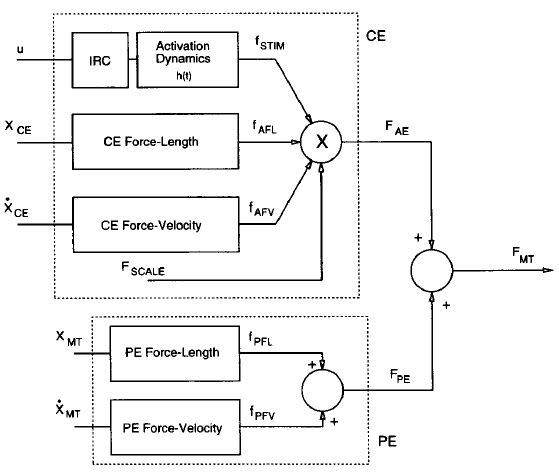
\includegraphics[width = 1\textwidth]{img/Durfee1994_Modelo.JPG}
\caption[Exemplo de Modelo Simplificado para Obter as Forças dos Músculos]{Modelo de um músculo eletricamente estimulado. A força proveniente do elemento CE é gerada por uma combinação multiplicativa de quatro fatores: ativação por estímulo, força-comprimento ativa, força-velocidade ativa e um fator de escala. A força proveniente do elemento PE é gerada por uma combinação somatória da força-comprimento passiva e da força-velocidade passiva 
\cite{durfee1994estimation}}
\label{modelo_durfee}
\end{figure}


\subsection{Forças de um Músculo a Partir de um Modelo Simplificado}
Como definido anteriormente, um modelo mais simplificado para se calcular a força líquida produzida por uma unidade motora pode ser descrito como em \cite{zajac1989muscle} onde a força é um resultado das propriedades força-comprimento e da força-velocidade, que estão dentro da dinâmica de contração. Em nosso modelo a entrada será a ativação dos elementos contráteis e a saída será a força produzida pela unidade motora, que pode ser extrapolada para um músculo inteiro.

O trabalho de \cite{zajac1989muscle} apresenta gráficos que definem o comportamento da força muscular $F^M$ em relação ao comprimento $l$ e a velocidade em que o músculo se deforma $v_m$. 

Os gráficos A e B definem uma propriedade estática do músculo e eles podem ser estudados quando o comprimento $L^M$ do músculo e o nível de ativação $a(t)$ são constantes. Uma ativação igual a 1 é considerada máxima quando os elementos contráteis do músculo forem excitados de forma máxima por muito tempo, ou seja, sem considerar mais o período transiente. Contrariamente um músculo é definido em repouso quando seu nível de ativação é 0, ou seja, inativo por muito tempo. A força identificada nos gráficos A e B é nomeada de força muscular ativa e esta força é gerada (nominalmente) entre $0,5{L_o}^M < L^M < 1,5{L_o}^M$, sendo ${L_o}^M$ o comprimento onde a força tem um pico (${F_o}^M$) \cite{zajac1989muscle}. Uma comparação entre os gráficos A e B mostra que músculos parcialmente ativados preservam as mesmas características que os músculos totalmente ativados.

Os gráficos C e D definem a propriedade da força-velocidade nos músculos. Quando um músculo é exposto a ativação máxima, ele fica sujeito a uma tensão constante, diminui e então para. O comprimento em que o músculo para então determina o comprimento no qual o músculo aguenta tal tensão no estado estático sob ativação máxima. Então os gráficos C e D podem ser utilizados para qualquer $L^M$ onde $0,5{L_o}^M < L^M < 1,5{L_o}^M$ \cite{zajac1989muscle}. Podemos retirar destes gráficos, então, qual a força $F^M$ que será exercida pelo músculo 

\begin{figure}[H]
\centering
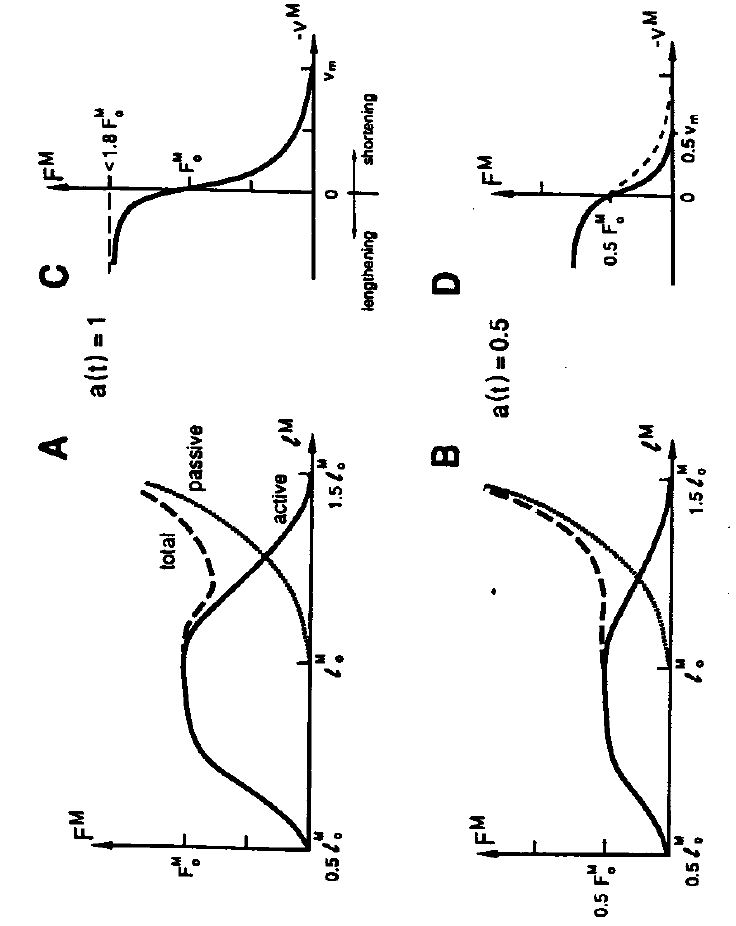
\includegraphics[width = 0.75\textwidth,angle=-90]{img/Zajac1989_Graficos.JPG}
\caption[Gráficos das propriedades força-comprimento e força-velocidade]{Propriedades do material dos tecidos musculares. (A e B) Propriedades estáticas
dos componentes passivo (PE) e ativo (CE) do músculo são dados através das curvas
normalizadas. $F^M$ e $L^M$ representam a força e o comprimento exercidos normalizados pelo
pico de força e pelo comprimento do músculo, respectivamente. (C e D) Propriedades
dinâmicas do músculo, do componente CE, é dada por uma relação adimensional entre
a força máxima que pode ser exercida e a velocidade do músculo. Note que $v_m$ também
é normalizado pelo máximo valor de $v_m$ do músculo. A amplitude das curvas C e D são
proporcionais ao nível de atuação (a), na curva C temos a = 1, na curva D temos a =
0,5.
\cite{zajac1989muscle}}
\label{graficos_zajac}
\end{figure}

As equações \ref{forcaCE} e \ref{forcaPE} no modelo de Hill demonstram as mesmas propriedades que as mostradas no gráfico \ref{graficos_zajac}. A força produzida pelo elemento PE depende somente do comprimento do músculo, enquanto a força produzida pelo elemento CE depende da $F_max$, do nivel de ativação a (ou $U$ na equação), e das propriedades força-comprimento e força-velocidade. Sendo assim é possível relacionar esses gráficos com aquelas equações estabelecidas anteriormente, sabendo que aqui pode-se determinar $F_max$ utilizando os gráficos C e D, que utilizam o nível de ativação e a velocidade com que o músculo se deforma. Portanto a curva estática do elemento ativo CE tem a amplitude modulada pela relação entre a ativação e a velocidade dada pela curva C, enquanto a curva estática do elemento passivo PE só depende do comprimento do músculo e tem um perfil exponencial.

Uma vez que o projeto será trabalhado no \textit{SIMULINK}, identificou-se uma facilidade em implementar o modelo a partir de uma interpolação das curvas determinadas por \cite{zajac1989muscle}. O \textit{MATLAB} foi utilizado para determinar polinômios capazes de representar de forma desejada as curvas descritas, os polinômios encontrados estão descritos em \ref{#1}

\begin{align}
F_{CE} = -0,8606x^5 + 12,39x^4 - 38,49x^3 + 43,6x^2 - 17,51x + 1,88 \label{funcCE} \\
F_{PE} = 8,13x^4 - 19x^3 + 15,07x^2 - 4,493x +0,3338 \label{funcPE}
F^M = F_{CE} + F_{PE} \label{funcFM}
F_{max} = 0,06757x^7 - 0,04067x^6 - 0,5223x^5 + 0,2424x^4 + 1,387x^3 - 0,4223x^2 - 1,844x + 1,12 \label{funcFMax}
\end{align}


% ---------------------------------------------------------------
%                                   CAPÍTULO 4
% ---------------------------------------------------------------
%\clearpage


\selectlanguage{Brazilian}

\chapter{RESULTADOS E DISCUSSÕES}\label{cap4}
A análise do resultado é feita a partir da validação da modelagem cinemática da mão e da ativação muscular. Em um primeiro momento estas são avaliadas separadamente, na seção \ref{resultado_cinematica} estão as avaliações feitas sobre os parâmetros de DH obtidos na seção \ref{cinematica_direta_mao} para condizerem com as restrições propostas na seção \ref{anatomia_mao}, e na seção \ref{resultado_ativacao} estão os gráficos de força, velocidade do músculo e ângulo da junta e como estes se relacionam ao proposto por \cite{zajac1989muscle}. Já na seção \ref{resultado_simulacao} está a integração entre os modelos apresentados e as discussões acerca dos resultados obtidos.
\section{Modelagem Cinemática da Mão}
\label{resultado_cinematica}
Para simplificação, nesta seção iremos abordar a modelagem dos dedos similares ao anelar, que possuem os mesmos parâmetros, diferente do dedo polegar. Levando em consideração as limitações da anatomia humana propostas por \cite{lin2000modeling} e os parâmetros de DH propostos na seção \ref{cinematica_direta_mao} para o dedo anelar é possível obter as relações entre os ângulos das articulações e a posição de cada junta enquanto o dedo se move. O modelo foi feito levando em consideração que este dedo possui uma junta diretiva e duas juntas flexivas, a representação dos ângulos $\theta$ estão nas figuras \ref{theta1} e \ref{thetas}. Nota-se como a representação das juntas é bem similar a apresentada por \cite{lee1995model} na figura \ref{Lee_Dedo}.

\begin{figure}[H]
\centering
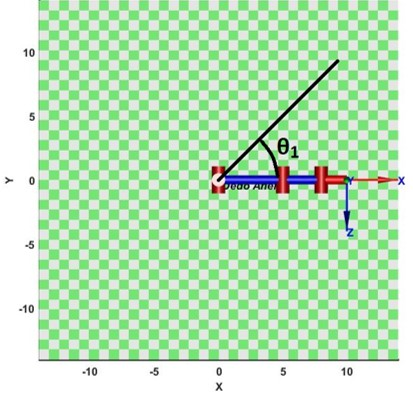
\includegraphics[width = 0.6\textwidth]{img/theta1.jpg}
\caption[Representação do ângulo $\theta_1$]{Representação do ângulo $\theta_1$}
\label{theta1}
\end{figure}

\begin{figure}[H]
\centering
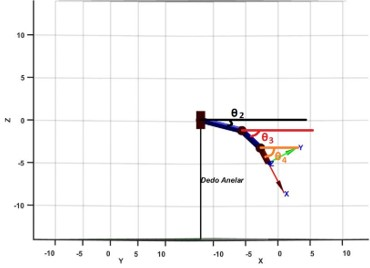
\includegraphics[width = 0.6\textwidth]{img/thetas.jpg}
\caption[Representação dos ângulos $\theta_2$, $\theta_3$ e $\theta_4$]{Representação dos ângulos $\theta_2$,$\theta_3$ e $\theta_4$}
\label{thetas}
\end{figure}

Correlacionando as juntas com as suas restrições, podemos destacar as restrições descritas para as juntas MP, PIP, DIP descritas na seção \ref{anatomia_mao}, e lembrando que o ângulo de flexão da junta DIP é relacionado ao ângulo da junta DIP como descrito em \ref{relacao_dip_pip}.
A partir dos parâmetros de DH é possível obter as matrizes de DH, onde pode-se obter as posições das juntas a partir dos ângulos em que as articulações estão dispostas. Mas é preciso determinar alguns parâmetros antes, como a distância entre as juntas, que, no dedo, seria representado pelo tamanho das falanges. Os parâmetros do tamanho das falanges foram obtidos através de medidas realizadas em algumas pessoas durante o projeto. Os parâmetros de tamanho de falange estão listados na tabela \ref{ParamResto} e as matrizes de DH para cada junta estão nas equações \ref{matriz_junta1}, \ref{matriz_junta2}, \ref{matriz_junta3} e \ref{matriz_junta4}.
As matrizes de cada junta em relação a junta anterior estão dispostas em \ref{junta1}, \ref{junta2}, \ref{junta3} e \ref{junta4} 
\begin{align}
A_1=
\begin{bmatrix}
cos_1 & 0 & -sen_1 & 0\\
sen_1 & 0 & cos_1 & 0\\
0 & -1 & 0 & 0\\
0 & 0 & 0 & 1\\
\end{bmatrix} \label{junta1}\\
A_2=
\begin{bmatrix}
cos_2 & -sen_2 & 0 & l1*cos_2\\
sen_2 & cos_2 & 0 & l1*sen_2\\
0 & 0 & 1 & 0\\
0 & 0 & 0 & 1\\
\end{bmatrix}  \label{junta2} \\
A_3=
\begin{bmatrix}
cos_3 & -sen_3 & 0 & l2*cos_3\\
sen_3 & cos_3 & 0 & l2*sen_3\\
0 & 0 & 1 & 0\\
0 & 0 & 0 & 1\\
\end{bmatrix}  \label{junta3} \\
A_4=
\begin{bmatrix}
cos_4 & -sen_4 & 0 & l3*cos_4\\
sen_4 & cos_4 & 0 & l3*sen_4\\
0 & 0 & 1 & 0\\
0 & 0 & 0 & 1\\
\end{bmatrix} \label{junta4}
\end{align}

\begin{align}
A_{MP_{AA}}= A_1 \label{matriz_junta1}\\
A_{MP_{F}}= A_1 * A_2 \label{matriz_junta2} \\
A_{PIP_{F}}= A_1 * A_2 * A_3 \label{matriz_junta3} \\
A_{DIP_{F}}= A_1 * A_2 * A_3 * A_4 \label{matriz_junta4}
\end{align}

Sendo $cos_i$ e $sen_i$ as representações de $cos(\theta_i)$ e $sen(\theta_i)$, e lembrando que $\theta_4 = \frac{2}{3}\theta_3$.

Com as tabelas é possível obter o posicionamento da junta em qualquer instante de tempo, dado os ângulos das juntas, estes provenientes do sistema de forças introduzido pelo modelo de Hill \cite{hill1938heat}. O posicionamento das juntas na tabela é descrito pela última coluna, onde as posições em cada eixo cartesiano é representado em uma linha, na linha 1 fica o valor do eixo x, na linha 2 fica o valor do eixo y e na linha 3 fica o valor do eixo z.

Para validar a restrição da angulação entre as juntas PIP e DIP foi simulado a resposta do dedo ao mover apenas a junta DIP, com uma entrada mostrada na figura \ref{ang_sim_pip}. A resposta para esta entrada está na figura \ref{sim_pip}, e é possível notar como a ângulação da junta DIP se move conforme a junta PIP porém com valores menores. Os ângulos para esta simulação foram retirados de medição empírica sobre dedos de algumas pessoas.

\begin{figure}[H]
\centering
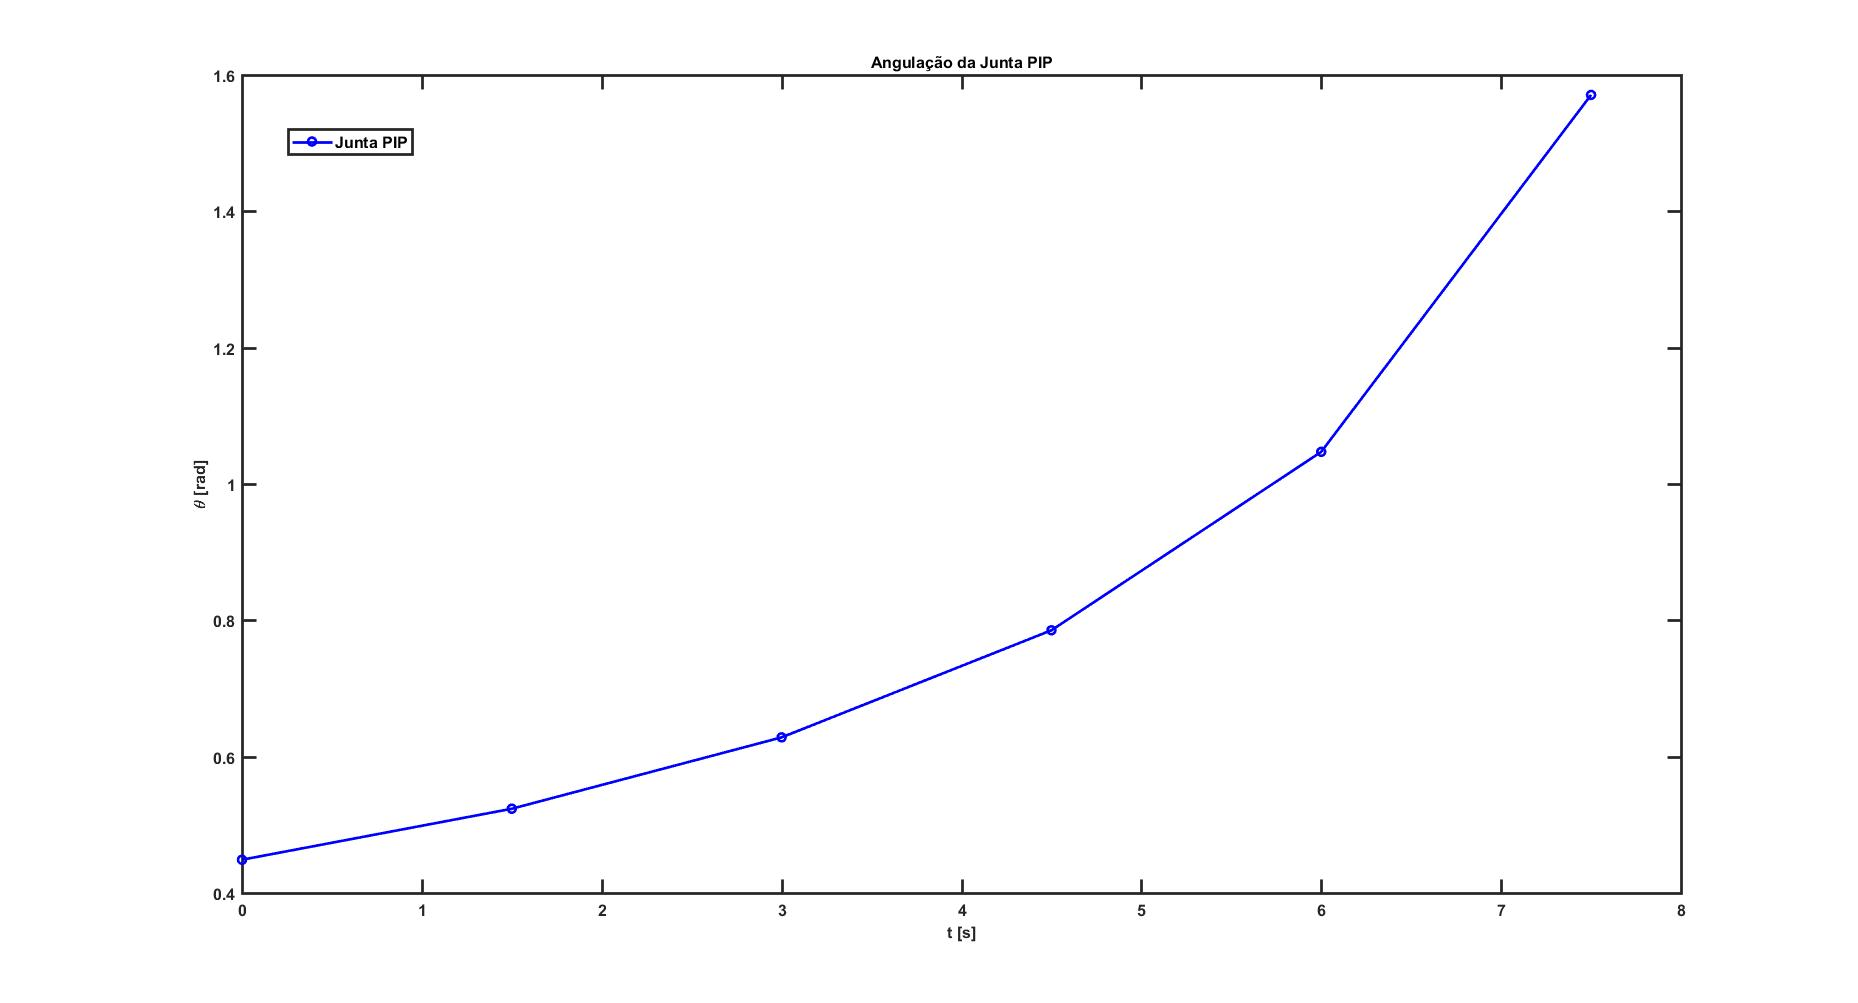
\includegraphics[width = 1\textwidth]{img/angulacao_pip.jpg}
\caption[Ângulos de simulação de entrada para a junta PIP]{Ângulos de simulação de entrada para a junta PIP}
\label{ang_sim_pip}
\end{figure}

\begin{figure}[H]
\centering
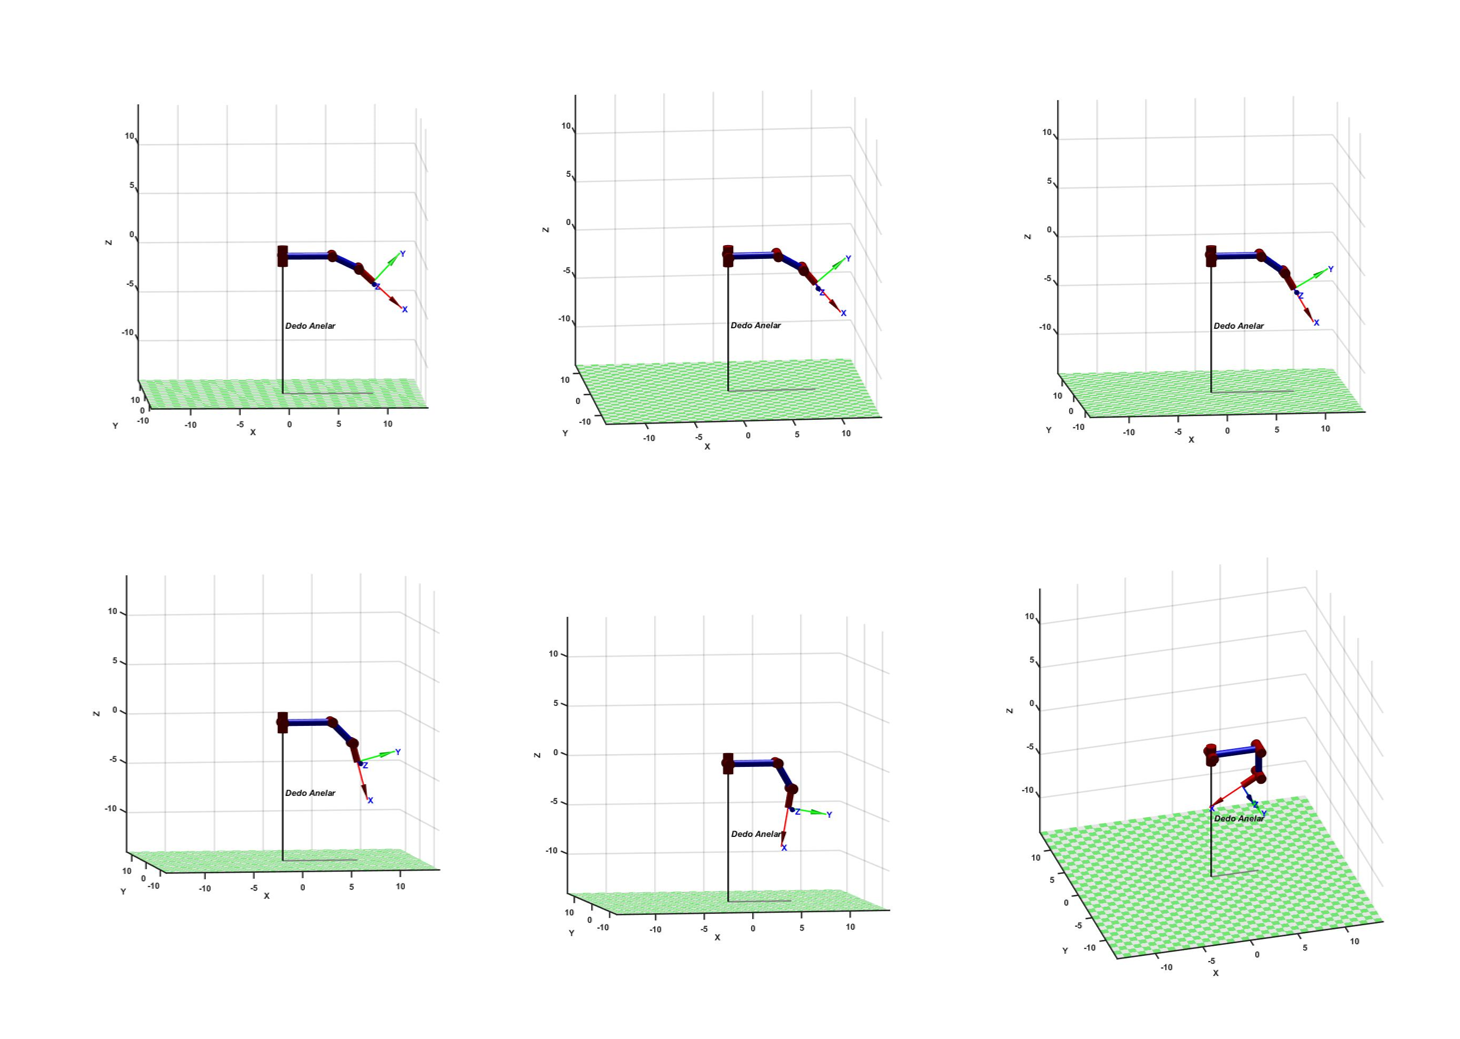
\includegraphics[width = 1\textwidth]{img/simpip.png}
\caption[Simulação de entrada para a junta PIP]{Simulação de entrada para a junta PIP}
\label{sim_pip}
\end{figure}

O mesmo é feito para a junta MP, onde foram aplicados os ângulos de entrada para os músculos de flexão e abudção/adução descritos na figura \ref{ang_sim_mp}. A resposta para esta entrada está na figura \ref{sim_mp}, onde é possível notar a movimentação das duas juntas e como o dedo se comporta quando estes músculos estão sobre força. Lembra-se que o ângulo de adução/abdução da junta MP é limitado em um range de $-15^\circ$ à $15^\circ$, por isso sua variação angular é pequena perto do ângulo de flexão. Os ângulos para esta simulação foram retirados de medição empírica sobre dedos de algumas pessoas.

\begin{figure}[H]
\centering
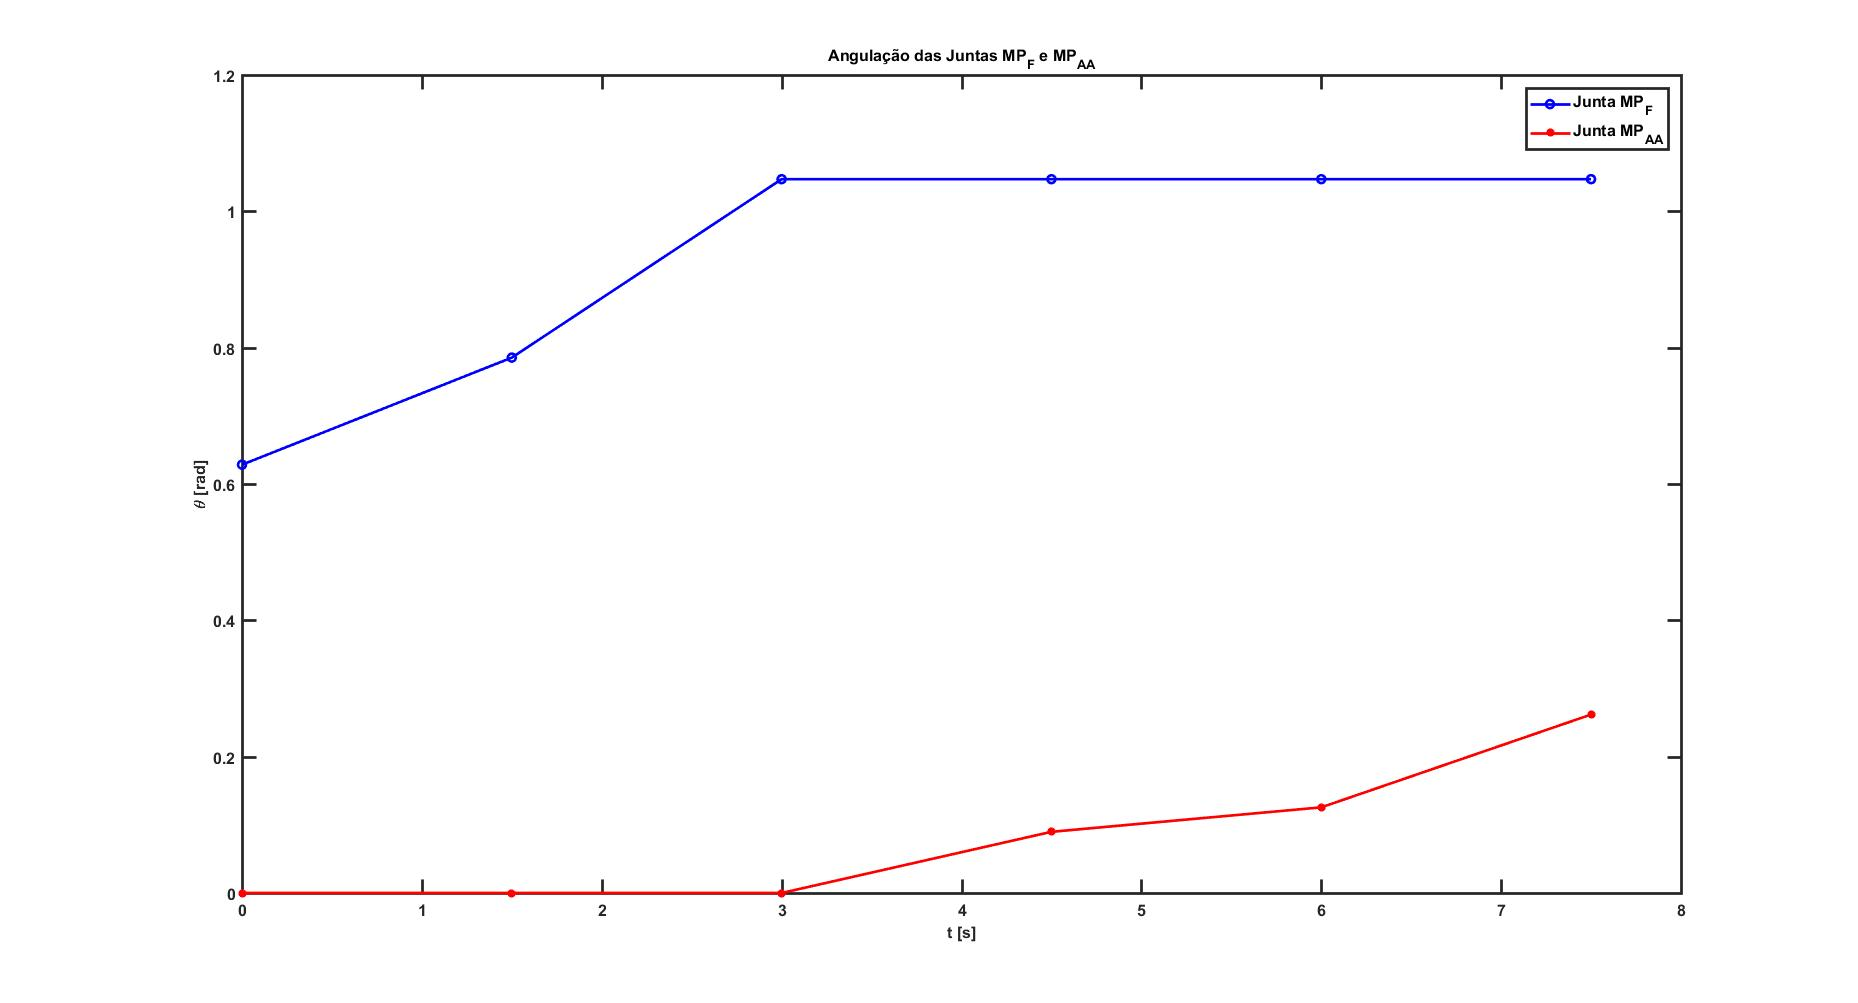
\includegraphics[width = 1\textwidth]{img/angulacao_mp.jpg}
\caption[Ângulos de simulação de entrada para a junta MP]{Ângulos de simulação de entrada para a junta MP}
\label{ang_sim_mp}
\end{figure}

\begin{figure}[H]
\centering
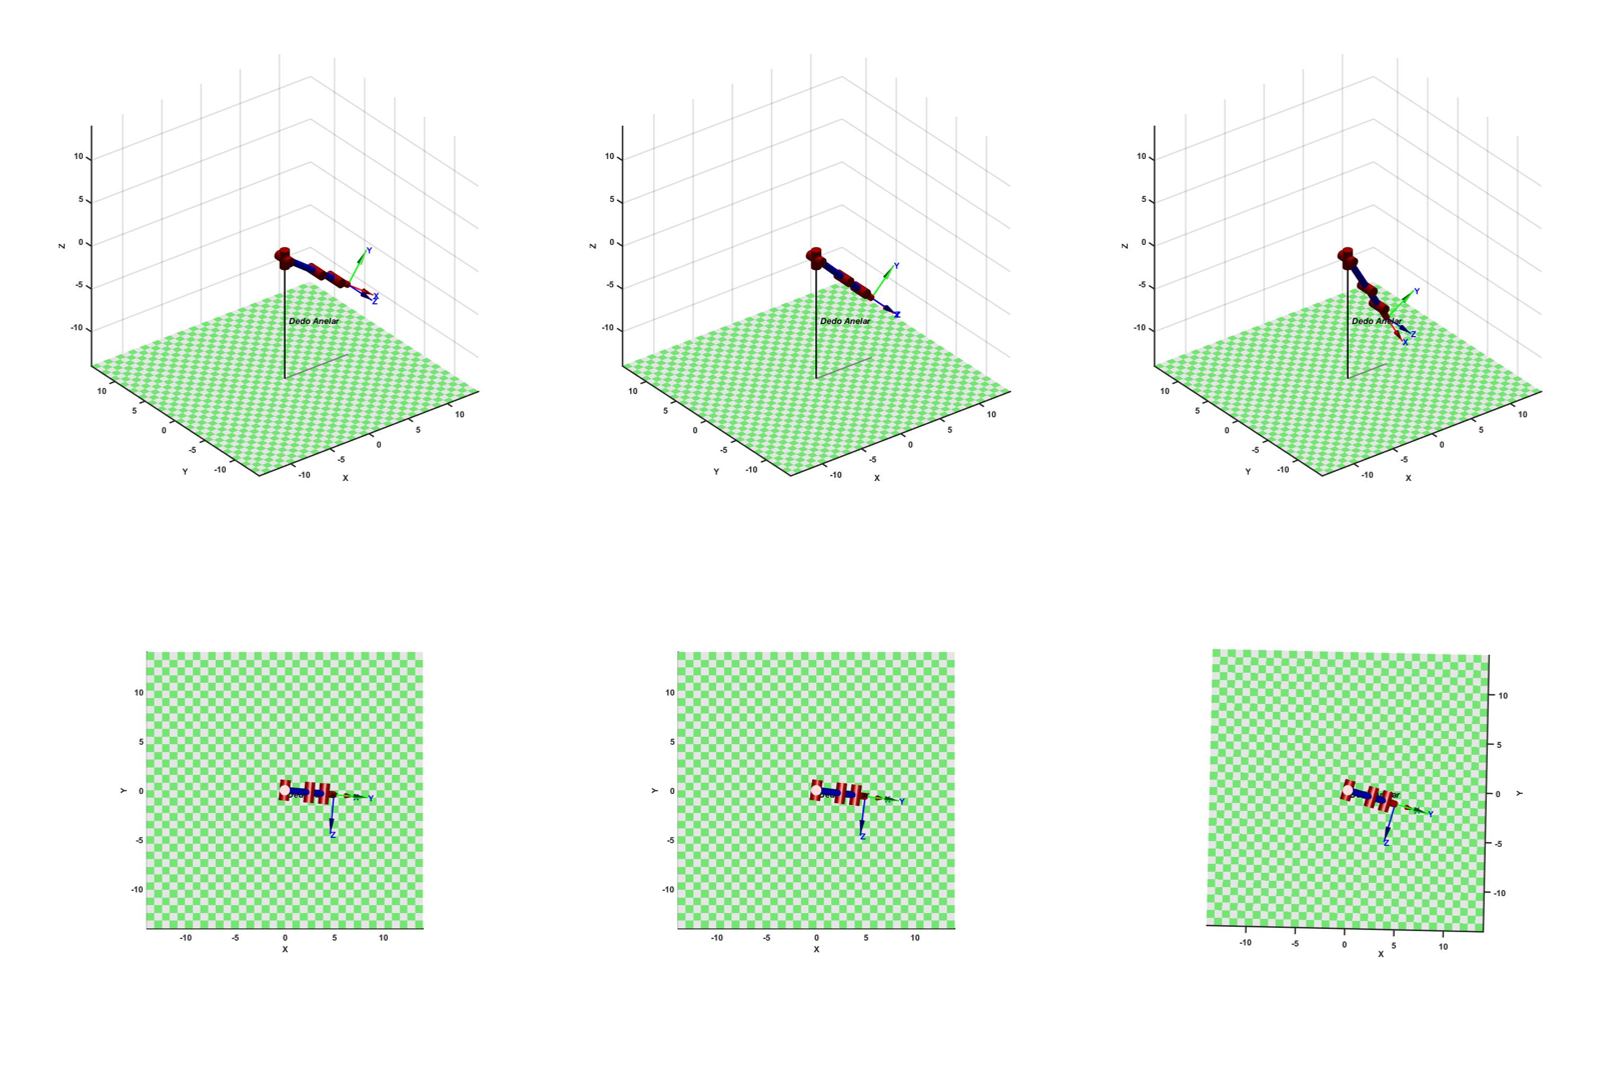
\includegraphics[width = 1\textwidth]{img/simmp.png}
\caption[Simulação de entrada para a junta MP]{Simulação de entrada para a junta MP}
\label{sim_mp}
\end{figure}

E por fim, uma simulação de todas as juntas estimuladas, demonstrando que as matrizes de DH representam bem o movimento de um dedo para as entradas da figura \ref{ang_sim_DH}. A figura \ref{sim_DH} representa a movimentação do dedo quando a entrada é a da figura \ref{ang_sim_DH}.

\begin{figure}[H]
\centering
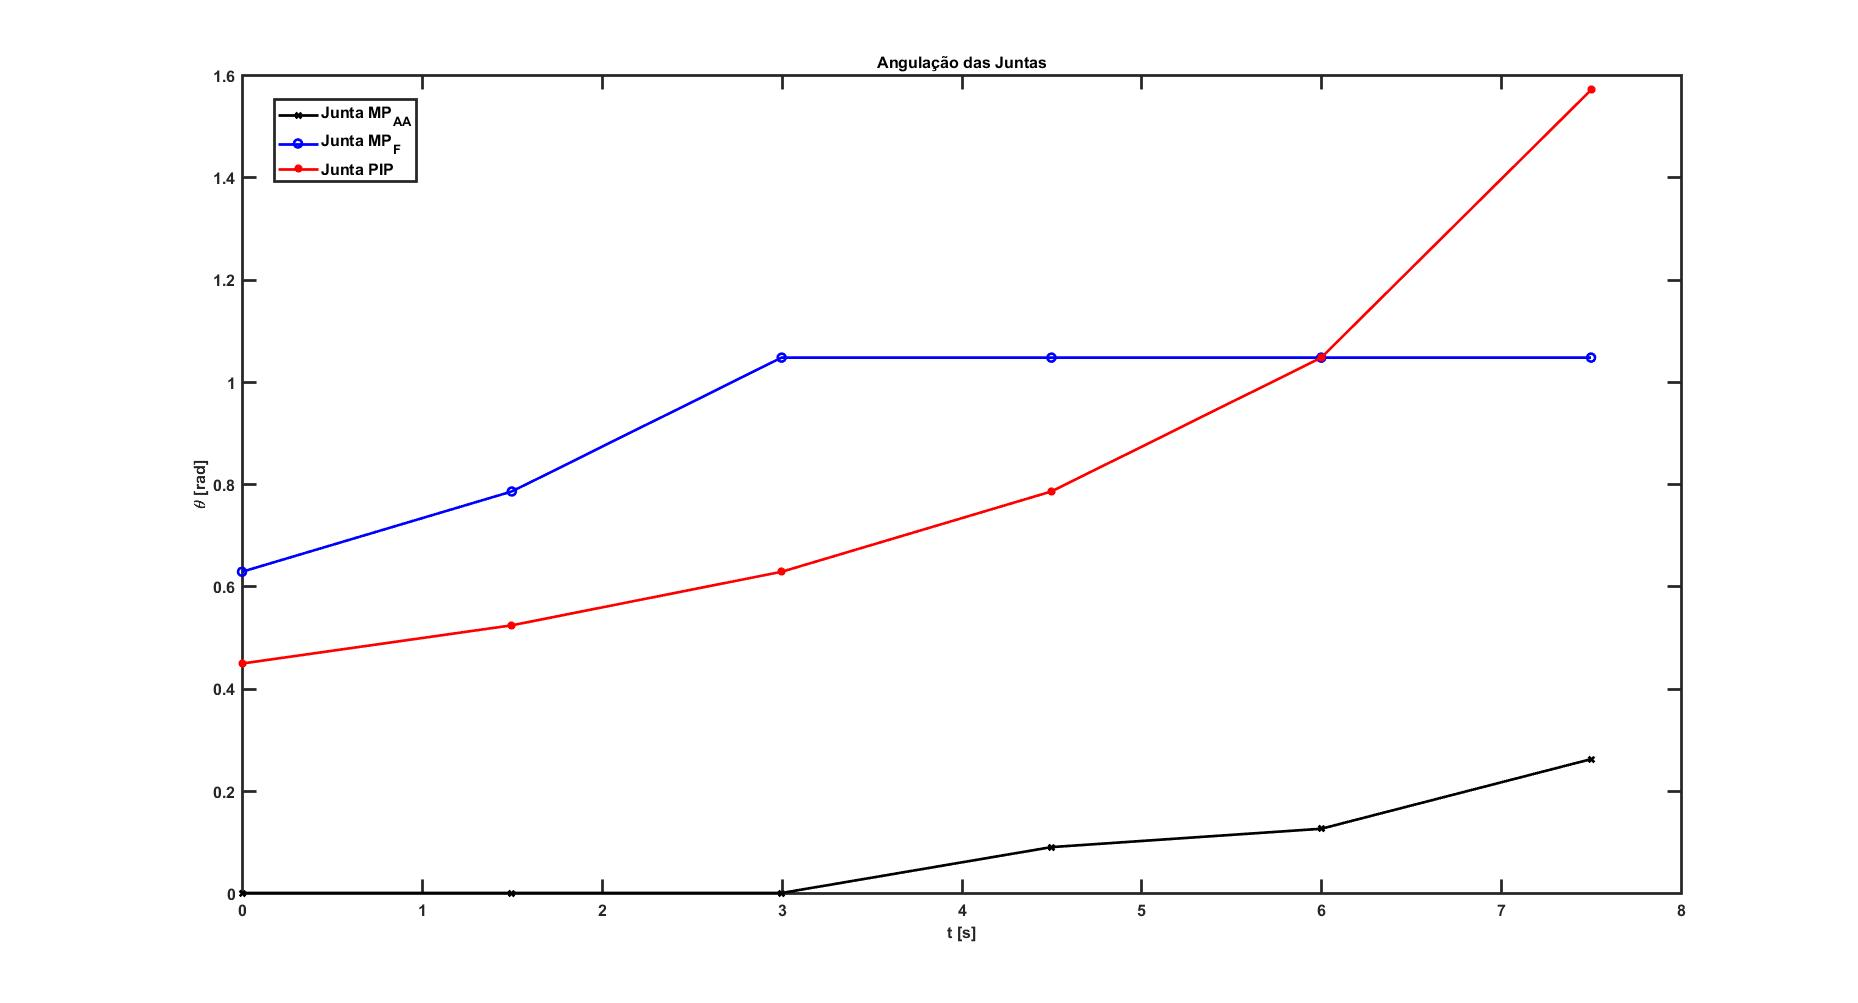
\includegraphics[width = 1\textwidth]{img/angulacao_tudo.jpg}
\caption[Ângulos de simulação de entrada para todas as juntas]{Ângulos de simulação de entrada para todas as juntas}
\label{ang_sim_DH}
\end{figure}

\begin{figure}[H]
\centering
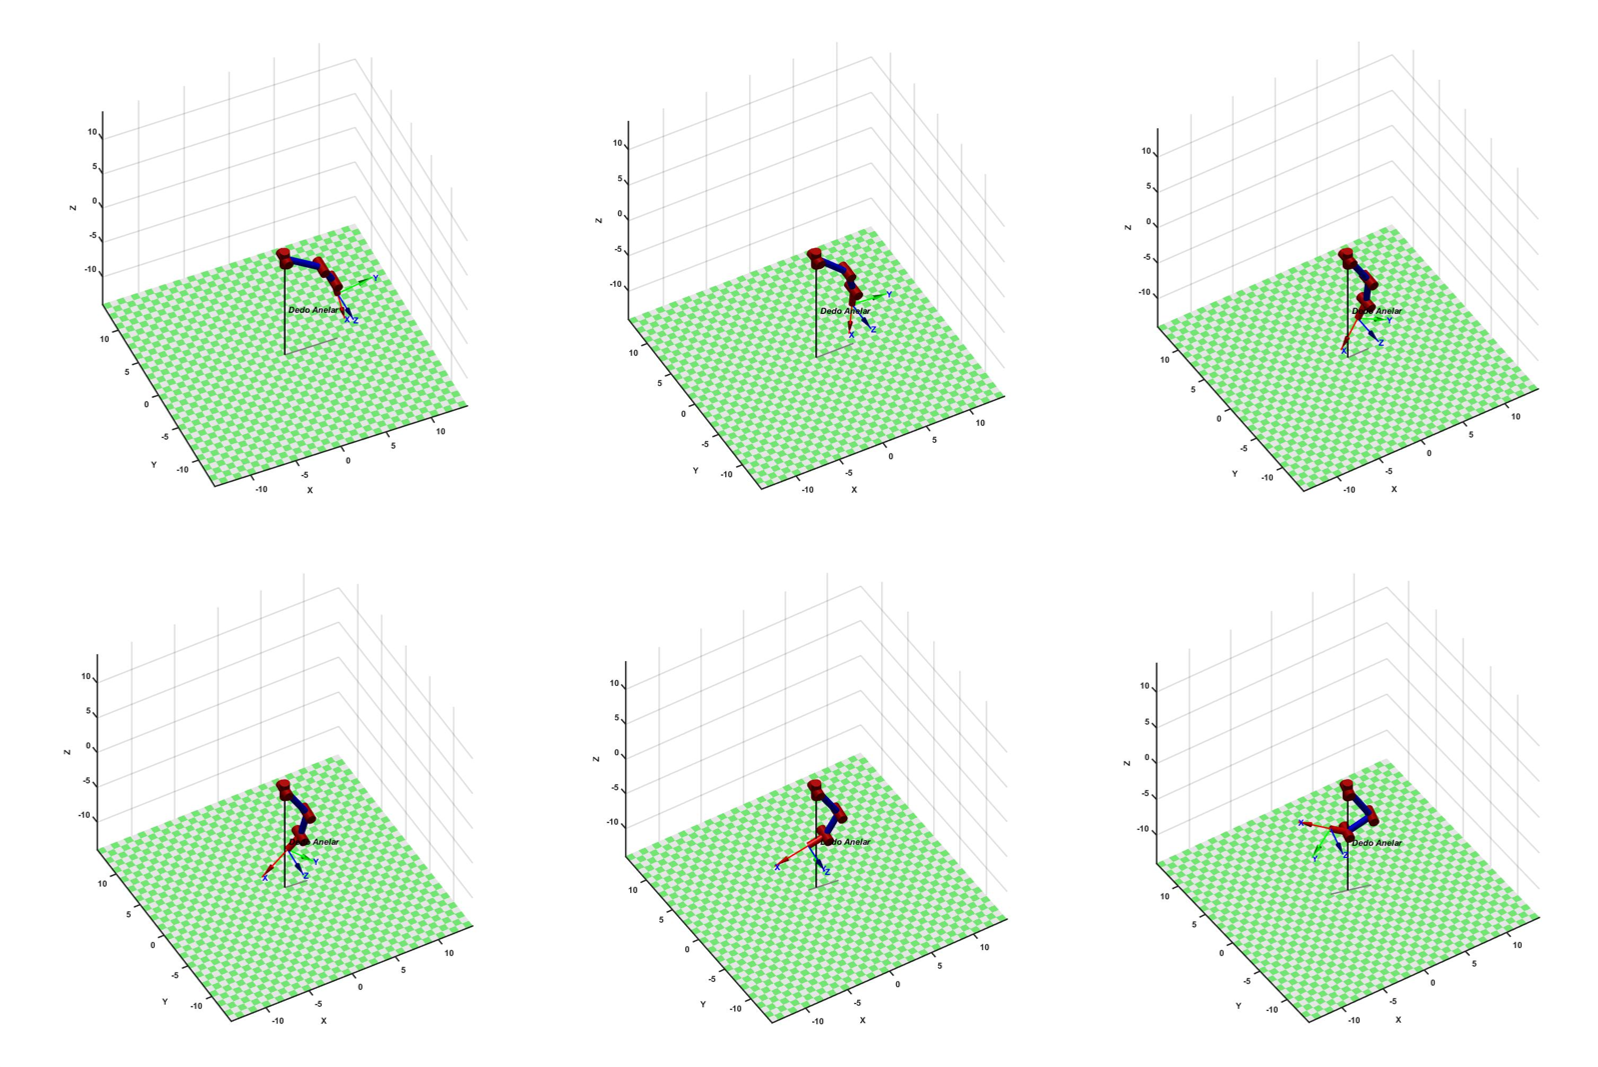
\includegraphics[width = 1\textwidth]{img/sim_total.png}
\caption[Simulação de entrada para todas as juntas]{Simulação de entrada para todas as juntas}
\label{sim_DH}
\end{figure}

\section{Modelagem da Ativação Muscular}
\label{resultado_ativacao}
Como explicado em \cite{zajac1989muscle} existem relações entre o nível de ativação muscular e o ângulo das articulações. Estas relações podem ser modeladas como foi proposto por \cite{feng1999surface} e mostrado na seção \ref{forcas_modelo_simplificado} é possível criar um modelo no \textit{SIMULINK} capaz de aproximar estas resoluções. O objetivo desta simulação é colher os dados de saída do modelo feito no \textit{SIMULINK} e compará-los aos de outros estudos como de \cite{zajac1989muscle}, \cite{rosen1999performances} e \cite{feng1999surface}. Para esta análise foi necessário definir algumas constantes empíricas para o funcionamento do modelo, como o MJG (da seção \ref{forcas_modelo_simplificado}) e os ângulos de repouso das juntas. Naturalmente, como evidenciado em \cite{lin2000modeling} os dedos da mão não ficam totalmente alinhados com o resto da mão quando em repouso, isso justifica as saídas de angulação da junta que não partem do $0^\circ$. 

Para este estudo o valor de MJG para as diferentes falanges está disposto na tabela \ref{MJG_tabela}, os diferentes valores foram obtidos de forma empírica enquanto se fazia o estudo, já que não foram encontrados valores conclusivos na literatura. O valor da geometria das articulações varia conforme as falanges devido, justamente, a geometria de cada falange, seu comprimento e circunferência são fatores que demonstram as diferenças neste parâmetro.

\begin{table}[H]
\centering
\caption{Tabela de Valores para MJG}
\label{MJG_tabela}
\begin{tabular}{|c|c|c|}
	\hline
    Falange & Valor de MJG (m) \\ \hline
    Falange próxima & 20 \\ \hline
    Falange média & 10 \\ \hline
    Falange distal & 5 \\
	\hline
\end{tabular}
\end{table}

Este valor, como proposto por \cite{feng1999surface} é o ganho que converte os torques exercidos pelos músculos em ângulos, velocidades e acelerações nas articulações.

Nesta simulação são feitos os movimentos de flexão e extensão de um músculo. Como este é um modelo normalizado, as respostas esperadas para estes movimentos podem ser aplicadas para os outros músculos dos dedos sem perda de coerência dos dados. Portanto esta simulação é feita sobre a falange próxima de um dedo da mão. Primeiramente, é executada a ação de flexionar o músculo colocando como entrada um nível de ativação máximo igual a 1, já que o modelo é normalizado. Assim que a ativação do movimento de flexão cessa, se inicia a ativação do músculo de extensão de mesma intensidade. O uso destes dois músculos foi previsto na seção \ref{integracao_validacao}, e ambas as forças dos músculos são dadas como positivas e então o sinal é alterado conforme o músculo atua como avanço ou recuo.

Os sinais utilizados para realizar os movimentos de flexão e extensão estão ilustrados na figura \ref{ativacao_musculos}.

\begin{figure}[H]
\centering
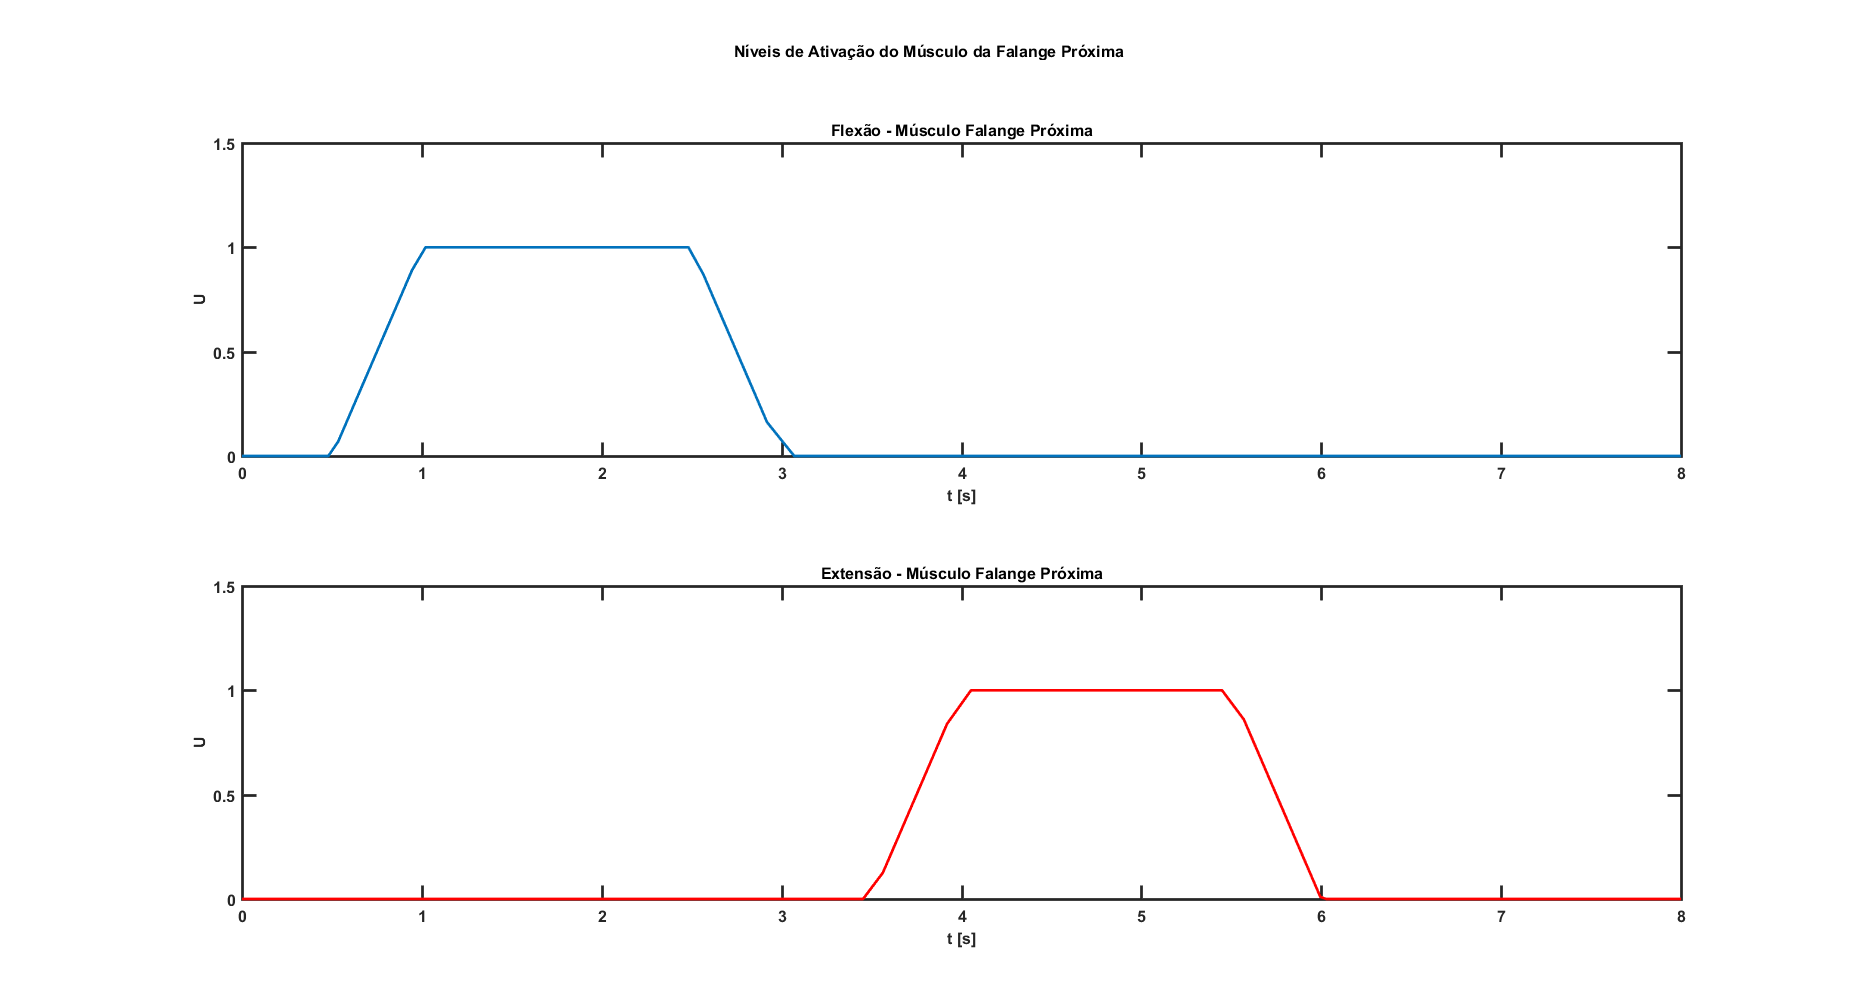
\includegraphics[width = 1\textwidth]{img/niveis_ativacao.png}
\caption[Níveis de Ativação para Flexão e Extensão para os Músculos de uma Falange Próxima]{Níveis de Ativação para Flexão e Extensão para os Músculos de uma Falange Próxima}
\label{ativacao_musculos}
\end{figure}

Ao excitar o músculo de flexão com um nível de ativação $U=1$ espera-se uma resposta condizente com as propostas por \cite{rosen1999performances}, onde a força do elemento CE depende do nível de atuação e a força do elemento PE não depende do nível de atuação, e sim do comprimento do músculo \cite{zajac1989muscle}. De início é feito a simulação como se só houvesse o movimento de flexão do músculo, para analisar qual é a resposta dos elementos de força do músculo e como seria a saída do modelo, em velocidade e ângulo. A figura \ref{sim_flexao} mostra o resultado da simulação de flexão pura. É possível notar que o elemento CE do músculo de flexão é ativado conforme o nível de ativação, e uma vez que este cessa o elemento CE não apresenta mais força, porém o elemento PE que possui sua saída de força atrelada ao comprimento do movimento, continua apresentando uma saída de força, justamente por que não houve uma extensão do músculo após a flexão, ou seja, o músculo continua "tensionado". É possível notar o mesmo comportamento no comprimento do músculo e na angulação de saída da junta, eles permanecem estáticos mesmo após o nível de atuação do movimento de flexão ter acabado.

\begin{figure}[H]
\centering
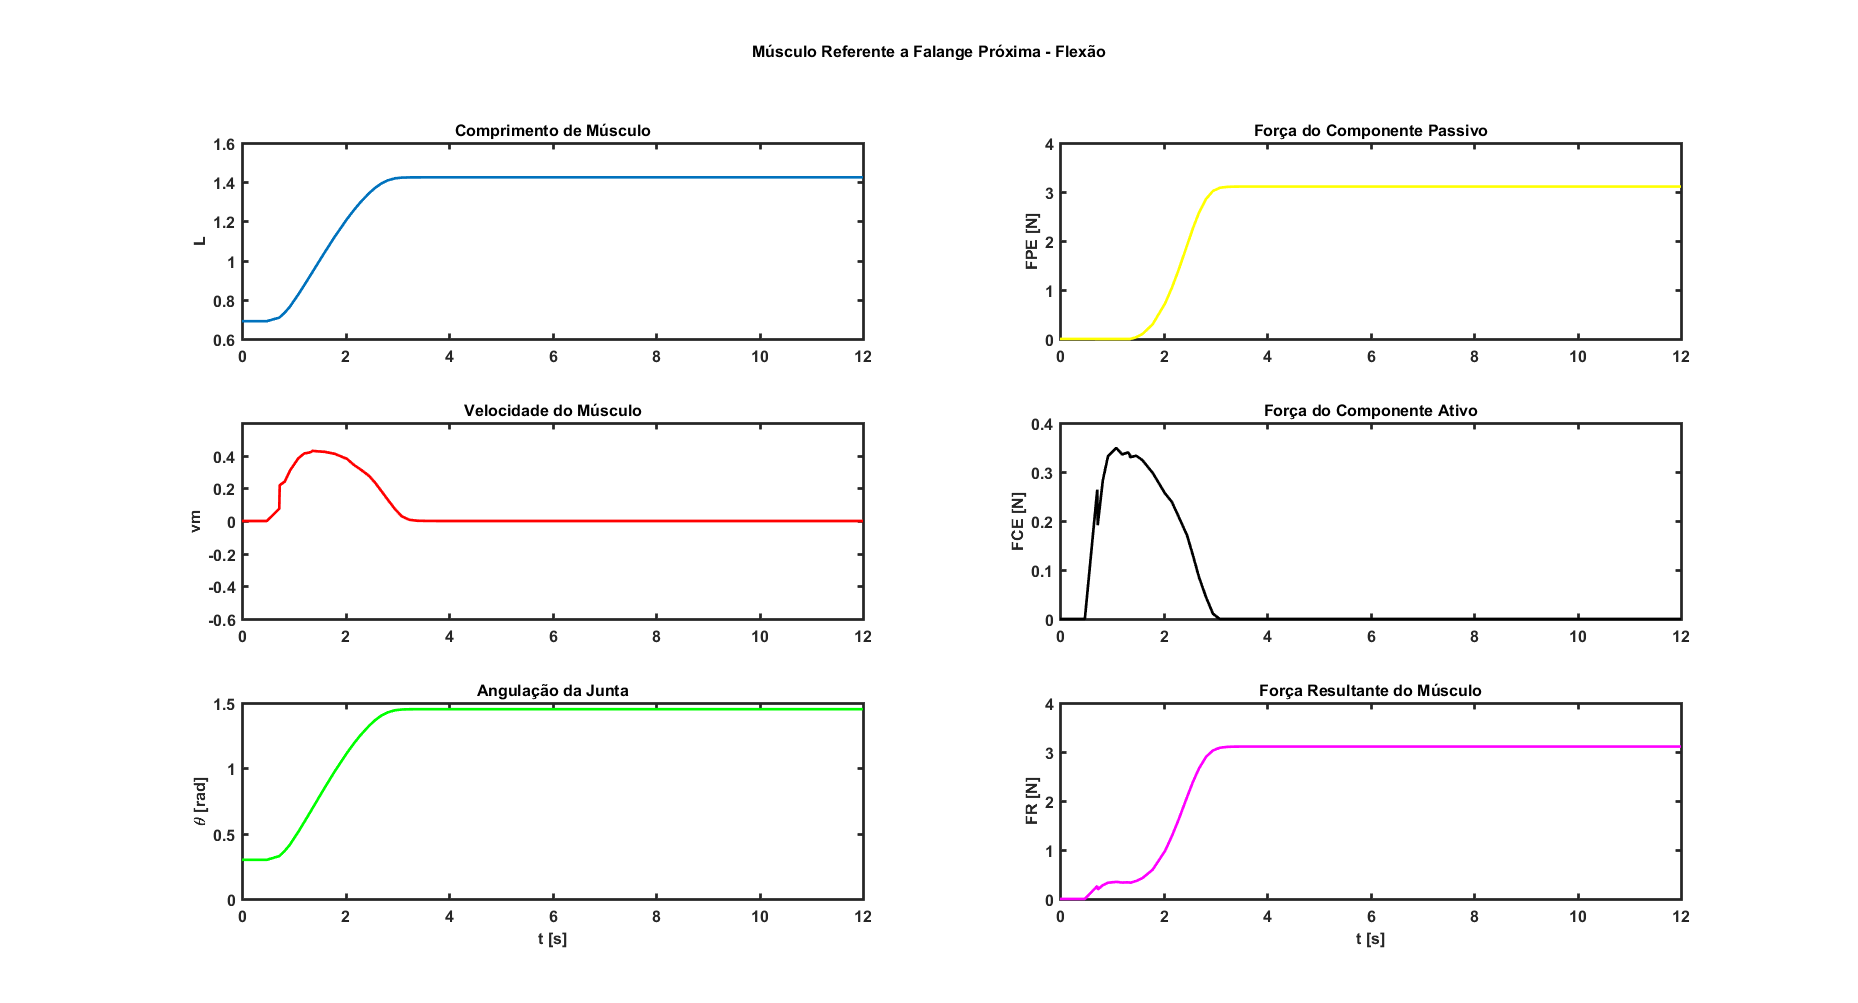
\includegraphics[width = 1\textwidth]{img/flexao.png}
\caption[Resposta ao Movimento de Flexão para uma Falange Próxima]{Resposta ao Movimento de Flexão para uma Falange Próxima}
\label{sim_flexao}
\end{figure}

Ao mesmo passo que o nível de ativação foi utilizado para uma flexão pura, é feito uma extensão no músculo assim que a flexão acaba. Com isso os níveis de atuação utilizados passam a ser exatamente os dois da figura \ref{ativacao_musculos}, já que antes era somente o primeiro destes. A resposta para um movimento de flexão e então extensão está ilustrado na figura \ref{sim_flexao_extensao}. Nesta resposta é possível notar que o movimento de extensão faz com que o comprimento do músculo volte a 0 e assim o elemento PE passa a não apresentar mais uma resposta de força. Sendo assim os outros parâmetros de saída do modelo acompanham e apresentam uma curva plausível com o movimento físico dos músculos.

\begin{figure}[H]
\centering
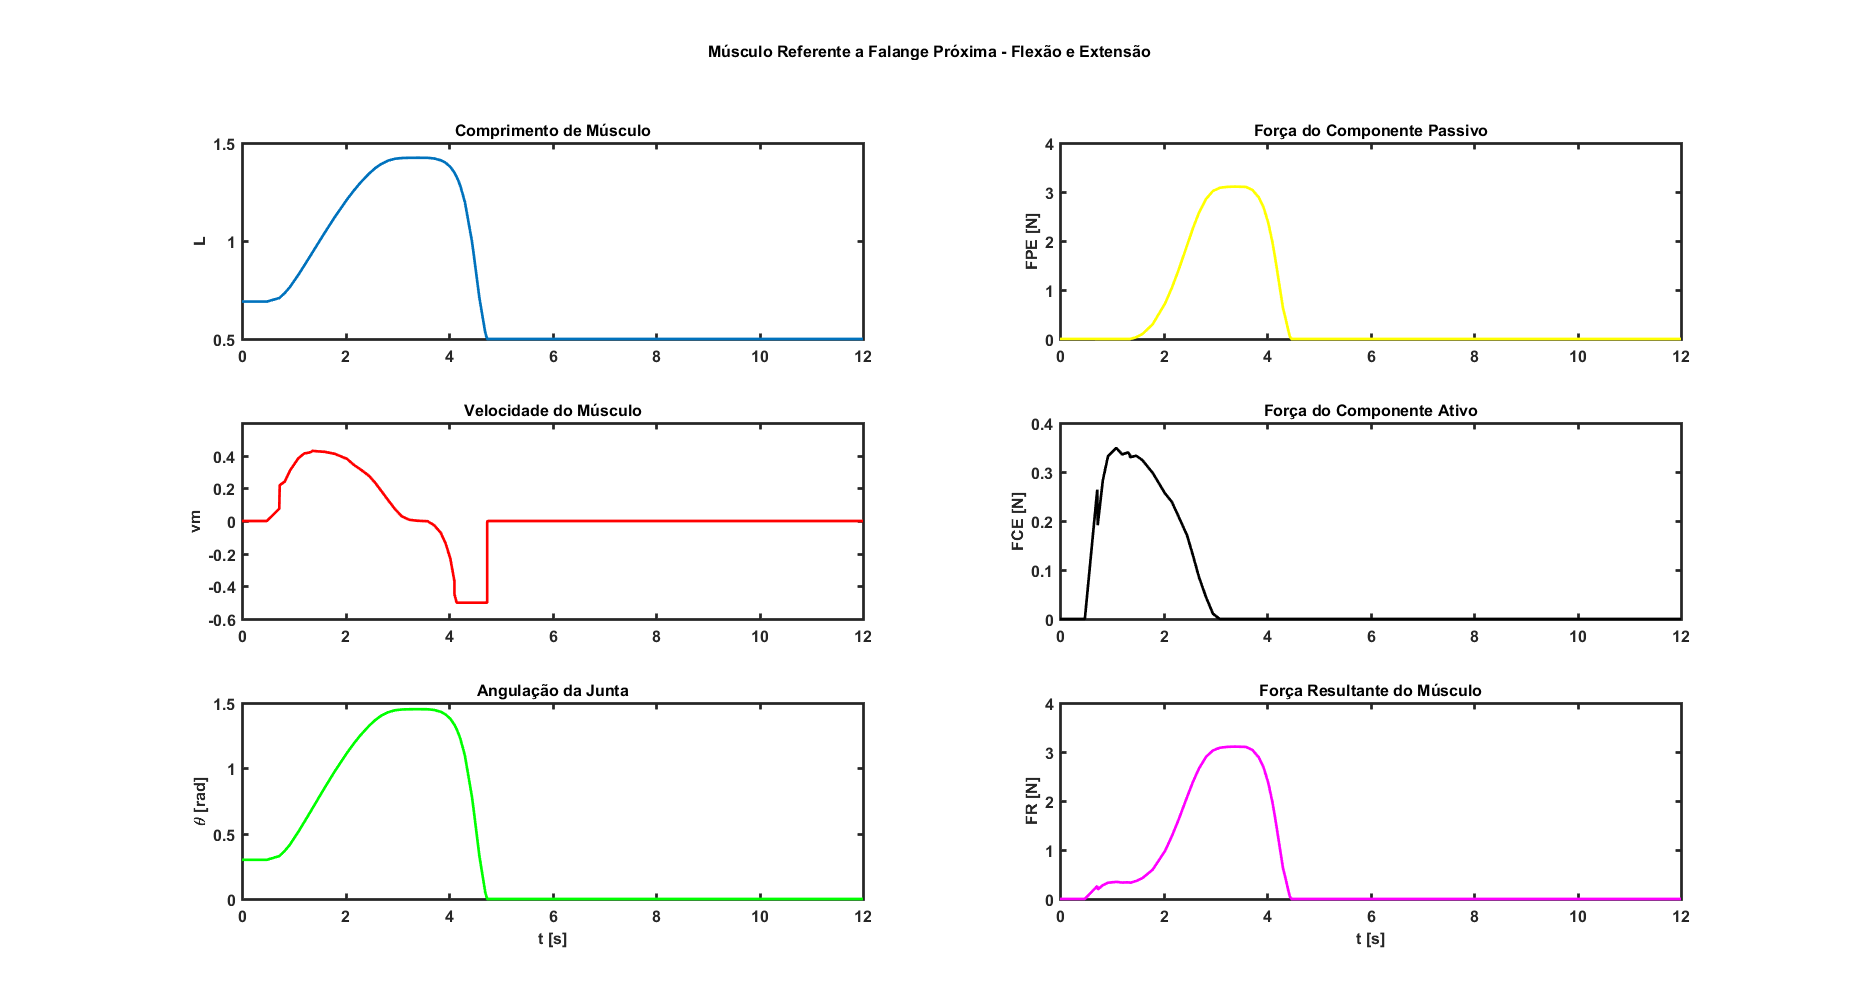
\includegraphics[width = 1\textwidth]{img/flexao_extensao.png}
\caption[Resposta ao Movimento de Flexão e em seguida Extensão para uma Falange Próxima]{Resposta ao Movimento de Flexão e em seguida Extensão para uma Falange Próxima}
\label{sim_flexao_extensao}
\end{figure}

Logo nota-se que, primeiramente o elemento CE responde diretamente ao nível de atuação, e a medida que o comprimento do músculo varia o elemento PE responde com uma força proporcional. Os maiores valores de $\theta$ são acompanhados do aumento da velocidade e normalmente ocorrem logo após estes, o que demonstra uma robustez física do modelo, assim como o fato de os movimentos opostos resultarem em um comprimento final tendendo a 0 para o músculo. 

Com um movimento completo de flexão e extensão, é possível correlacionar as curvas de ângulo da junta e velocidade com as obtidas por \cite{rosen1999performances}, demonstradas na figura \ref{rosen_ativacao}. Lembra-se que o estudo performado por \cite{rosen1999performances} se tratava de uma captura de dados utilizando a tecnologia sEMG, a qual possui ruídos, os quais não existem nestas simulações, já que foram feitas utilizando curvas ideais produzidas pelo \textit{MATLAB}.

\begin{figure}[H]
\centering
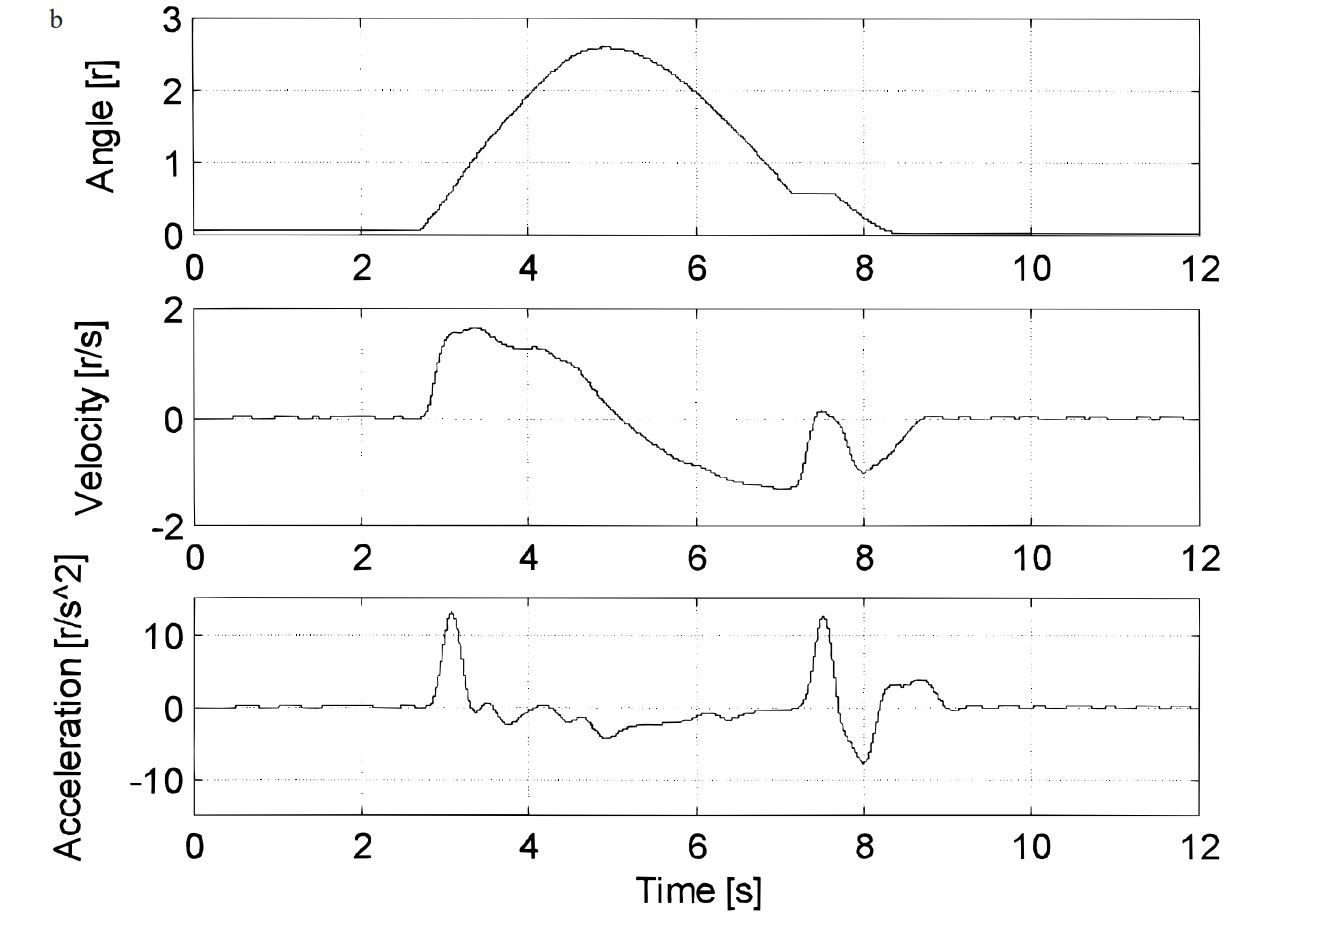
\includegraphics[width = 1\textwidth]{img/Rosen1999_ativacao.JPG}
\caption[Resposta ao Movimento de Flexão seguido de Extensão em um Ombro]{Registros de uma sessão típica. Cinemática do ombro : ângulo da articulação do ombro, velocidade angular, e aceleração angular \cite{rosen1999performances}}
\label{rosen_ativacao}
\end{figure}

\section{Simulação do Movimento Completo}
\label{resultado_simulacao}

\subsection{Movimento Completo}

% ---------------------------------------------------------------
%                                   CAPÍTULO 5
% ---------------------------------------------------------------
%\clearpage


\selectlanguage{Brazilian}

\chapter{CONCLUSÃO}\label{cap5}
Este projeto visava mostrar a relação entre o modelo de Hill descrito por \cite{hill1938heat} e a cinemática direta da mão de um ser humano. O projeto baseou-se em trabalhos como os de \cite{zajac1989muscle}, \cite{lee1995model}, \cite{feng1999surface} e \cite{rosen1999performances}, para analisar e validar a integração entre as ativações musculares e a cinemática da mão.

Analisando os resultados obtidos no capítulo \ref{cap4} pode-se dizer que as integrações entre os modelos se deu de forma satisfatória, já que os músculos respondiam corretamente aos níveis de atuação e durante as simulações era possível notar o crescimento da velocidade conforme os músculos eram excitados. Todas as validações no capítulo \ref{cap4} valem para os outros dedos da mão e do dedo polegar, bastando corrigir os valores de MJG para os diferentes de dedos, e no caso do polegar, ainda, as matrizes de DH são diferentes devido aos parâmetros de DH serem diferentes. Sendo assim a vantagem do modelo obtido neste projeto reside no nível de atuação, e os parâmetros do músculo estarem normalizados, portanto as respostas se limitam as restrições físicas do dedo e parâmetros como MJG.

O objetivo futuro para este estudo consiste em fazer uma modelagem mais completa da mão levando em consideração outras restrições como descritas em \cite{lee1995model}, e como os dedos interagem com a palma da mão, onde existem novos graus de liberdade para todos os dedos. E aprimorar o modelo de Hill construído para que este fique mais robusto.




% ---------------------------------------------------------------
%                          REFERÊNCIAS
% ---------------------------------------------------------------
\clearpage


\bibliographystyle{apalike}         
\bibliography{referencias}



% ---------------------------------------------------------------
%                                            ANEXO
% ---------------------------------------------------------------
% %\cleardoublepage
% \clearpage

% \let\originalanexo=\anexo
% % \def\anexo{\cleardoublepage\originalanexo}
% \renewcommand*{\theHsection}{\thepart.\thesection}

% \setcounter{chapter}{0}
% \def\thechapter{\Alph{chapter}}

% \phantomsection
% \addcontentsline{toc}{chapter}{ANEXOS}
% %%% Anexo A
% \begin{center}
	\anexo{-- \ \ Título do Anexo}\label{AnexoA}
\end{center}

Os dados apresentados a seguir correspondem os arquivos de entrada utilizados para testar o problema de geração de vorticidade em escoamento ar/líquido...\\

\section{Título}\label{AnexoA:1}

O arquivo a seguir apresenta as configurações...

\clearpage



% -----------------------------------------------------------------------------
%                                           APÊNDICE
% -----------------------------------------------------------------------------
% %\cleardoublepage 
% \clearpage

% \let\originalappendix=\appendix
% % \def\appendix{\cleardoublepage\originalappendix}

% \setcounter{chapter}{0}
% \def\thechapter{\Alph{chapter}}

% \phantomsection
% \addcontentsline{toc}{chapter}{APÊNDICES}
% %%% Apêndice A
% \begin{center}
\appendix{-- \ \ Título do Apêndice}\label{ApendiceA}
\end{center}

\textcolor{Blue}{Os apêndices (e também os anexos) são identificados por letras maiúsculas consecutivas, travessão e pelos respectivos títulos.}\\

\section{Parte 1}\label{ApendiceA:1}

%\lstinputlisting[]{./apendices/sources/file.XXX}



     % Usando input fez o "APÊNDICES" apareçer no lugar certo no sumario
% %%%

\end{document}
